\documentclass[11pt,a4paper]{article}

% French
\usepackage[utf8x]{inputenc}
\usepackage[frenchb]{babel}
\usepackage[T1]{fontenc}
\usepackage{lmodern}
\usepackage{ifthen}

% Color
% cfr http://en.wikibooks.org/wiki/LaTeX/Colors
\usepackage{color}
\usepackage[usenames,dvipsnames,svgnames,table]{xcolor}
\definecolor{dkgreen}{rgb}{0.25,0.7,0.35}
\definecolor{dkred}{rgb}{0.7,0,0}

% Floats and referencing
\newcommand{\sectionref}[1]{section~\ref{sec:#1}}
\newcommand{\annexeref}[1]{annexe~\ref{ann:#1}}
\newcommand{\figuref}[1]{figure~\ref{fig:#1}}
\newcommand{\tabref}[1]{table~\ref{tab:#1}}
\usepackage{xparse}
\NewDocumentEnvironment{myfig}{mm}
{\begin{figure}[!ht]\centering}
{\caption{#2}\label{fig:#1}\end{figure}}

% Listing
\usepackage{listings}
\lstset{
  numbers=left,
  numberstyle=\tiny\color{gray},
  basicstyle=\rm\small\ttfamily,
  keywordstyle=\bfseries\color{dkred},
  frame=single,
  commentstyle=\color{gray}=small,
  stringstyle=\color{dkgreen},
  %backgroundcolor=\color{gray!10},
  %tabsize=2,
  rulecolor=\color{black!30},
  %title=\lstname,
  breaklines=true,
  framextopmargin=2pt,
  framexbottommargin=2pt,
  extendedchars=true,
  inputencoding=utf8x
}

\newcommand{\matlab}{\textsc{Matlab}}
\newcommand{\octave}{\textsc{GNU/Octave}}
\newcommand{\qtoctave}{\textsc{QtOctave}}
\newcommand{\oz}{\textsc{Oz}}
\newcommand{\java}{\textsc{Java}}
\newcommand{\clang}{\textsc{C}}
\newcommand{\keyword}{mot clef}

% Math symbols
\usepackage{amsmath}
\usepackage{amssymb}
\usepackage{amsthm}
\DeclareMathOperator*{\argmin}{arg\,min}
\DeclareMathOperator*{\argmax}{arg\,max}

% Sets
\newcommand{\Z}{\mathbb{Z}}
\newcommand{\R}{\mathbb{R}}
\newcommand{\Rn}{\R^n}
\newcommand{\Rnn}{\R^{n \times n}}
\newcommand{\C}{\mathbb{C}}
\newcommand{\K}{\mathbb{K}}
\newcommand{\Kn}{\K^n}
\newcommand{\Knn}{\K^{n \times n}}

% Chemistry
\newcommand{\std}{\ensuremath{^{\circ}}}
\newcommand\ph{\ensuremath{\mathrm{pH}}}

% Theorem and definitions
\theoremstyle{definition}
\newtheorem{mydef}{Définition}
\newtheorem{mynota}[mydef]{Notation}
\newtheorem{myprop}[mydef]{Propriétés}
\newtheorem{myrem}[mydef]{Remarque}
\newtheorem{myform}[mydef]{Formules}
\newtheorem{mycorr}[mydef]{Corrolaire}
\newtheorem{mytheo}[mydef]{Théorème}
\newtheorem{mylem}[mydef]{Lemme}
\newtheorem{myexem}[mydef]{Exemple}
\newtheorem{myineg}[mydef]{Inégalité}

% Unit vectors
\usepackage{esint}
\usepackage{esvect}
\newcommand{\kmath}{k}
\newcommand{\xunit}{\hat{\imath}}
\newcommand{\yunit}{\hat{\jmath}}
\newcommand{\zunit}{\hat{\kmath}}

% rot & div & grad & lap
\DeclareMathOperator{\newdiv}{div}
\newcommand{\divn}[1]{\nabla \cdot #1}
\newcommand{\rotn}[1]{\nabla \times #1}
\newcommand{\grad}[1]{\nabla #1}
\newcommand{\gradn}[1]{\nabla #1}
\newcommand{\lap}[1]{\nabla^2 #1}


% Elec
\newcommand{\B}{\vec B}
\newcommand{\E}{\vec E}
\newcommand{\EMF}{\mathcal{E}}
\newcommand{\perm}{\varepsilon} % permittivity

\newcommand{\bigoh}{\mathcal{O}}
\newcommand\eqdef{\triangleq}

\DeclareMathOperator{\newdiff}{d} % use \dif instead
\newcommand{\dif}{\newdiff\!}
\newcommand{\fpart}[2]{\frac{\partial #1}{\partial #2}}
\newcommand{\ffpart}[2]{\frac{\partial^2 #1}{\partial #2^2}}
\newcommand{\fdpart}[3]{\frac{\partial^2 #1}{\partial #2\partial #3}}
\newcommand{\fdif}[2]{\frac{\dif #1}{\dif #2}}
\newcommand{\ffdif}[2]{\frac{\dif^2 #1}{\dif #2^2}}
\newcommand{\constant}{\ensuremath{\mathrm{cst}}}

% Numbers and units
\usepackage[squaren, Gray]{SIunits}
\usepackage{sistyle}
\usepackage[autolanguage]{numprint}
%\usepackage{numprint}
\newcommand\si[2]{\numprint[#2]{#1}}
\newcommand\np[1]{\numprint{#1}}

\newcommand\strong[1]{\textbf{#1}}
\newcommand{\annexe}{\part{Annexes}\appendix}

% Bibliography
\newcommand{\biblio}{\bibliographystyle{plain}\bibliography{biblio}}

\usepackage{fullpage}
% le `[e ]' rend le premier argument (#1) optionnel
% avec comme valeur par défaut `e `
\newcommand{\hypertitle}[7][e ]{
\usepackage{hyperref}
{\renewcommand{\and}{\unskip, }
\hypersetup{pdfauthor={#6},
            pdftitle={Synth\`ese d#1#2 Q#3 - L#4#5},
            pdfsubject={#2}}
}

\title{Synth\`ese d#1#2 Q#3 - L#4#5}
\author{#6}

\begin{document}

\ifthenelse{\isundefined{\skiptitlepage}}{
\begin{titlepage}
\maketitle

 \paragraph{Informations importantes}
   Ce document est grandement inspiré de l'excellent cours
   donné par #7 à l'EPL (École Polytechnique de Louvain),
   faculté de l'UCL (Université Catholique de Louvain).
   Il est écrit par les auteurs susnommés avec l'aide de tous
   les autres étudiants, la vôtre est donc la bienvenue.
   Il y a toujours moyen de l'améliorer, surtout si le cours
   change car la synthèse doit alors être modifiée en conséquence.
   On peut retrouver le code source à l'adresse suivante
   \begin{center}
     \url{https://github.com/Gp2mv3/Syntheses}.
   \end{center}
   On y trouve aussi le contenu du \texttt{README} qui contient de plus
   amples informations, vous êtes invité à le lire.

   Il y est indiqué que les questions, signalements d'erreurs,
   suggestions d'améliorations ou quelque discussion que ce soit
   relative au projet
   sont à spécifier de préférence à l'adresse suivante
   \begin{center}
     \url{https://github.com/Gp2mv3/Syntheses/issues}.
   \end{center}
   Ça permet à tout le monde de les voir, les commenter et agir
   en conséquence.
   Vous êtes d'ailleurs invité à participer aux discussions.

   Vous trouverez aussi des informations dans le wiki
   \begin{center}
     \url{https://github.com/Gp2mv3/Syntheses/wiki}.
   \end{center}
   comme le statut des synthèses pour chaque cours
   \begin{center}
     \url{https://github.com/Gp2mv3/Syntheses/wiki/Status}.
   \end{center}
   vous pouvez d'ailleurs remarquer qu'il en manque encore beaucoup,
   votre aide est la bienvenue.

   Pour contribuer au bug tracker et au wiki, il vous suffira de
   créer un compte sur Github.
   Pour interagir avec le code des synthèses,
   il vous faudra installer \LaTeX.
   Pour interagir directement avec le code sur Github,
   vous devez utiliser \texttt{git}.
   Si cela pose problème,
   nous sommes évidemment ouverts à des contributeurs envoyant leurs
   changements par mail ou n'importe quel autre moyen.
\end{titlepage}
}{}

\ifthenelse{\isundefined{\skiptableofcontents}}{
\tableofcontents
}{}
}


\usepackage[utf8x]{inputenc}
\usepackage{ucs}
\usepackage{amsmath}
\usepackage{amsfonts}
\usepackage{amssymb}
\usepackage{graphicx}
\usepackage{color}


\hypertitle{Dispositifs Electroniques: Synthèse des tuyaux partie Bayot}{5}{ELEC}{1330}
{Initial: Albert de Jamblinne, Relecture :Nicolas Van der Noot 2011 \\ Ajoute et correction: Destrée Maxime 2012}
{Vincent Bayot et Denis Flandre}

\newpage

Résolution  des question tuyaux avec synthèse du cours.
Notation : les vecteurs sont notés en gras; si il ne le sont pas, on sous entend que c'est la norme de ceux-ci.
\section{Question 1}
Décrire la relation de dispersion d'un cristal unidimensionnel infini, pour les modèles de Sommerfeld et Kronig et Penney. Quelles sont les conséquences sur la vitesse de groupe et la masse des électrons ? Calculer la contribution au courant d'une bande pleine d'électrons.
\\
\hbox{\raisebox{0.4em}{\vrule depth 0pt height 0.4pt width 6cm}}
\\
\subsection{Hypotèses du modèle }
\begin{enumerate}
\item Le modèle est dérivé à une dimension, mais est généralisable à 3 dimensions.
\item Pour éviter les problèmes aux limites, on considère un cristal infini. 
\item On considère un cristal parfait constitué de N noyaux et de P électrons.
\item On néglige les vibrations de réseau, ce qui revient à considérer que les noyaux sont fixes et que la position de ceux-ci est donc connue.
\item Approximation de Hartree-Fock: Le cristal est électriquement neutre  (à l'échelle macroscopique), et est considéré comme un ensemble d'ions (fixes, dont la position est connue) et d'électrons quasi-libres. Les ions sont constitués des noyaux et des électrons de cœur, les électrons quasi-libres sont les électrons de valence.
\item Tout les électrons sont indépendants, ils n'interagissent pas entre eux.
\item La seul interaction entre les électrons et le cristal est due à un potentiel $V(x)$, comprenant l'influence des noyau et des électrons  de coeur. Ce potentiel est donné par la figure (c) ci-dessous.\\
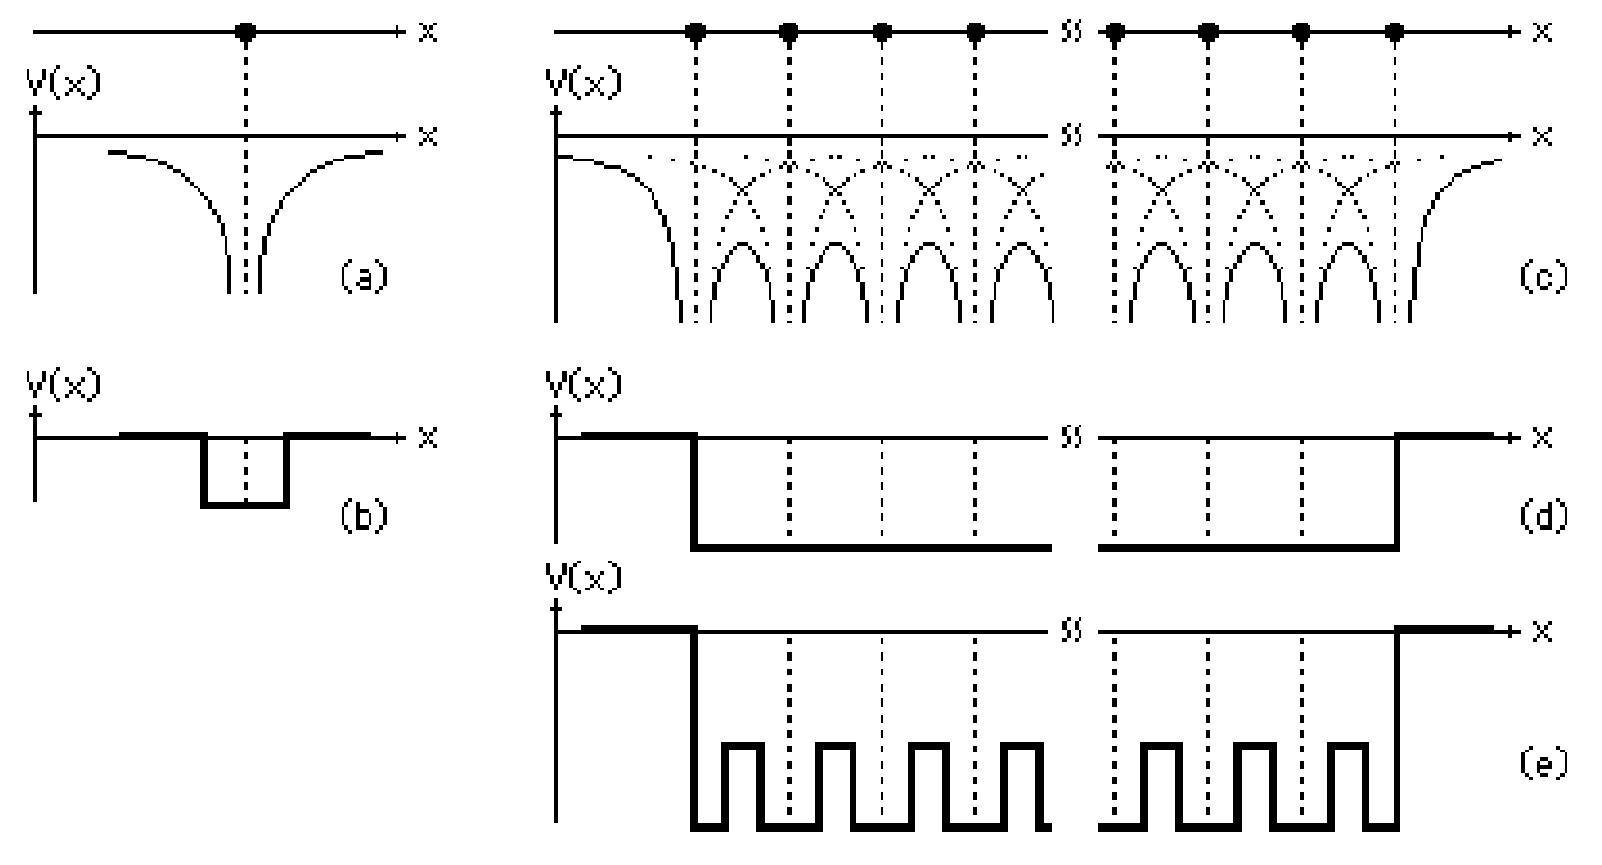
\includegraphics[scale=0.4]{vx.eps} \\
\subsection{relation de dispersion}
La résolution des équations de Schrödinger avec ce potentiel est très compliquée. Pour simplifier, on peut utiliser les potentiels décrits par les figures (d) et (e). (d) représente le modèle de Sommerfeld et consiste à ne considérer qu'un puits de potentiel moyen sur tout le cristal. (e) est le potentiel utilisé pour le modèle de Krönig et Penney. Une description plus formelle de ce potentiel est donnée par la figure ci-dessous. On notera que le potentiel V(x) est périodique, ce qui implique que la solution de Schrödinger est, à priori, une fonction de Bloch. \\
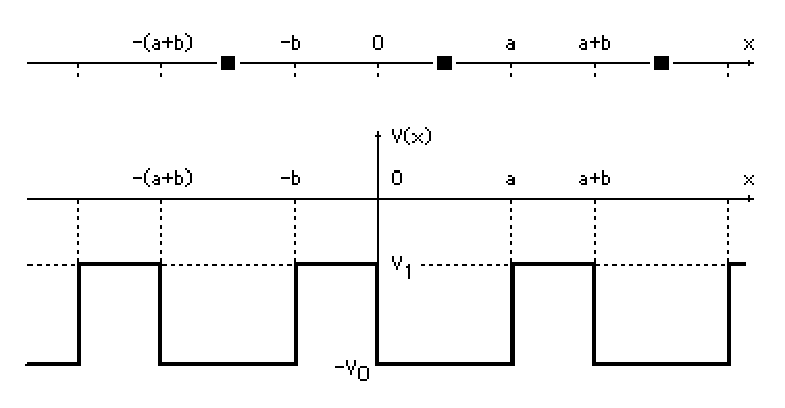
\includegraphics[scale=0.8]{cronig.eps} \\
\end{enumerate}
Le modèle de Sommerfield est un cas particulier du modèle de Krönig et Penney. En effet, si la barrière de potentiel tend vers zéro, on retrouve le modèle de Sommerfield. Considérons donc le modèle de Krönig et Penney. On a un potentiel crénelé, le fond du puits de potentiel est à $V(x)=-V_0$ et le haut de la barrière de potentiel est à $V(x)=V_1$. La largeur du puits est 'a' et la largeur de la barrière est 'b'. Pour simplifier les expressions de l'équation de dispersion, on définit  'm' la masse de l'électron et 'E' l'énergie totale de l'électron.  On démarre de l'équation de Schrödinger :
\begin{eqnarray}
- \frac{\hbar^2}{2m} \frac{d^2 \Phi(x)}{dx^2} - V_0 \Phi(x) = E \Phi(x) & \ \mbox{pour } \ & \ 0 \leq x \leq a \\ 
- \frac{\hbar^2}{2m} \frac{d^2 \Phi(x)}{dx^2} + V_1 \Phi(x) = E \Phi(x) & \ \mbox{pour } \ & \ -b < x < 0 \\ 
\end{eqnarray}
Les solutions sont des exponentielles fonction de :
\begin{equation}
\alpha=\frac{1}{\hbar}\sqrt[2]{2m(E+V_0)}
\end{equation}
\begin{equation}
\beta=\frac{1}{\hbar}\sqrt[2]{2m(V_1-E)}
\end{equation}
La résolution s'effectue en posant les conditions limite de périodicité et de continuité de $\Phi(0)$. Dans le puits ($0\leq x \leq a$); on trouve une somme d'exponentielles complexes, c'est-à-dire une fonction oscillante comme une particule libre; hors du puits ($-b\leq x\leq 0$), on obtient une exponentielle décroissante qui témoigne de l'effet tunnel.
%La relation de dispersion ainsi obtenue est :
%\begin{equation}
%cos[k(a+b)]=cos[\alpha a]cosh[\beta b]+ \frac{b(\beta^2-\alpha^2)}{2\alpha}sin(\alpha a)\frac{sinh(\beta b)}{\beta b}
%\end{equation}
On peut simplifier le modèle en considérant que les barrières de potentiel sont très hautes ($V_1 \rightarrow \infty$) et très étroites ($b\rightarrow 0$), mais en conservant néanmoins une valeur finie pour le produit $V_1~b$. On obtient finalement comme relation de dispersion :% On obtiens alors que $\beta b ~,~ b\alpha^2 \rightarrow 0$ et que $b\beta^2$ est non nul.
%\begin{equation}
%\underbrace{cos[k(a+b)]}_{=cos(ka)}=cos[\alpha a]\underbrace{cosh[\beta b]}_{=1}+ \frac{b(\beta^2-\alpha^2)}{2\alpha}sin(\alpha a)\underbrace{\frac{sinh(\beta b)}{\beta b}}_{=1}
%\end{equation}
%\begin{equation}
%cos(ka)=cos[\alpha a]+\frac{b(\beta^2)}{2\alpha}sin(\alpha a)
%\end{equation}
%or $b(\beta^2)=b\frac{1}{\hbar^2} 2mV_1$, ce terme caractérise la transparence de la barrière de potentiel, Pour simplifier, on pose dès lors : $P=\frac{abV_1m}{\hbar^2} $ et on obtient :
\begin{equation}
cos(ka)=cos(\alpha a)+P \frac{sin(\alpha a)}{\alpha a}
\end{equation}
avec $P=\frac{abV_1m}{\hbar^2} $.

Le terme de droite ne peut prendre que des valeurs comprise entre $-1$ et $1$. Cela limite donc l'ensemble des valeurs de $\alpha a$ qui sont solutions de l'équation.
Si on isole $E$ dans l'expression de $\alpha$, on peut tracer le graphe de $E$ en fonction de $\alpha a$ (une parabole) et y reporter les valeurs possibles trouvées précédemment. On voit alors apparaître une alternance de bandes d'énergie permises et interdites.Finalement, on peut dessiner $E(ka)$ ; le spectre ainsi obtenu pour l'énergie en fonction du vecteur d'onde est :
\\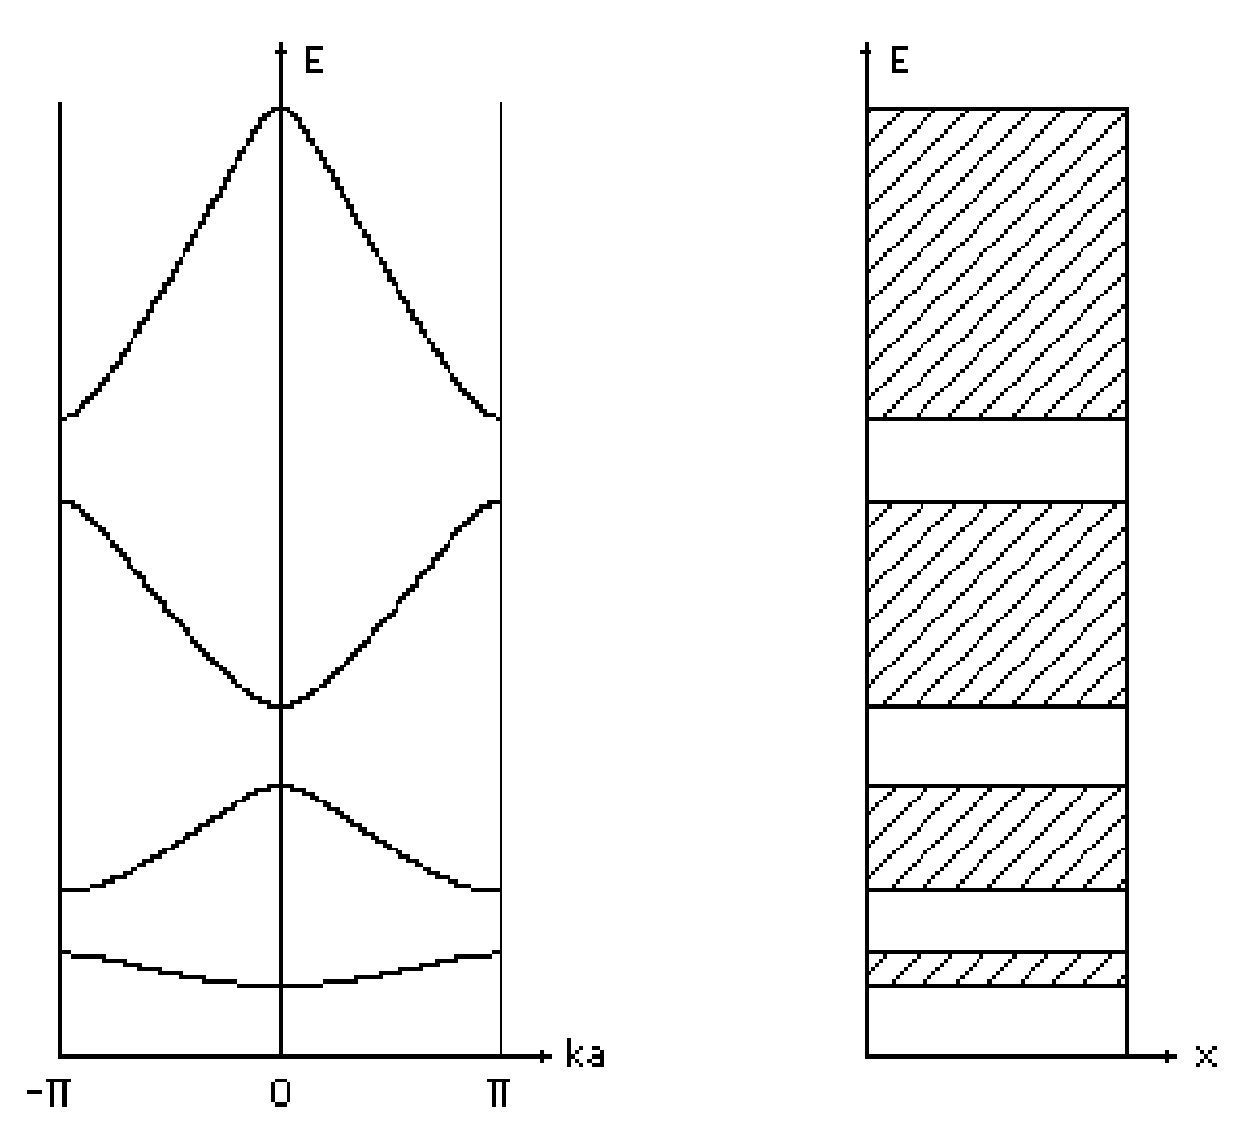
\includegraphics[scale=0.4]{disp.eps} \\
On remarque d'abord que la fonction de dispersion est périodique (période de $\pi/a$ et paire $(E(k)=E(-k))$. On ne représente donc la fonction que pour une seule période, c'est à dire pour les vecteurs d'onde qui se situent dans la première zone de Brillouin $k \in [-\pi/a ; \pi/a]$.% On voit ensuite qu'il y a apparition de bandes continues d'énergie, alternées par des bandes interdites.\\

Le cas particulier de P=0 correspond au modèle de Sommerfeld. Le fonction de dispersion est alors donnée par :
\begin{equation}
cos(ka)=cos(\alpha a)
\end{equation}
ce qui est en fait, dans le cas d'un cristal infini, le modèle de l'électron libre. Pour la première bande d'énergie, le graphe obtenu (en comparaison avec le cas P différent de zéro) est:
\\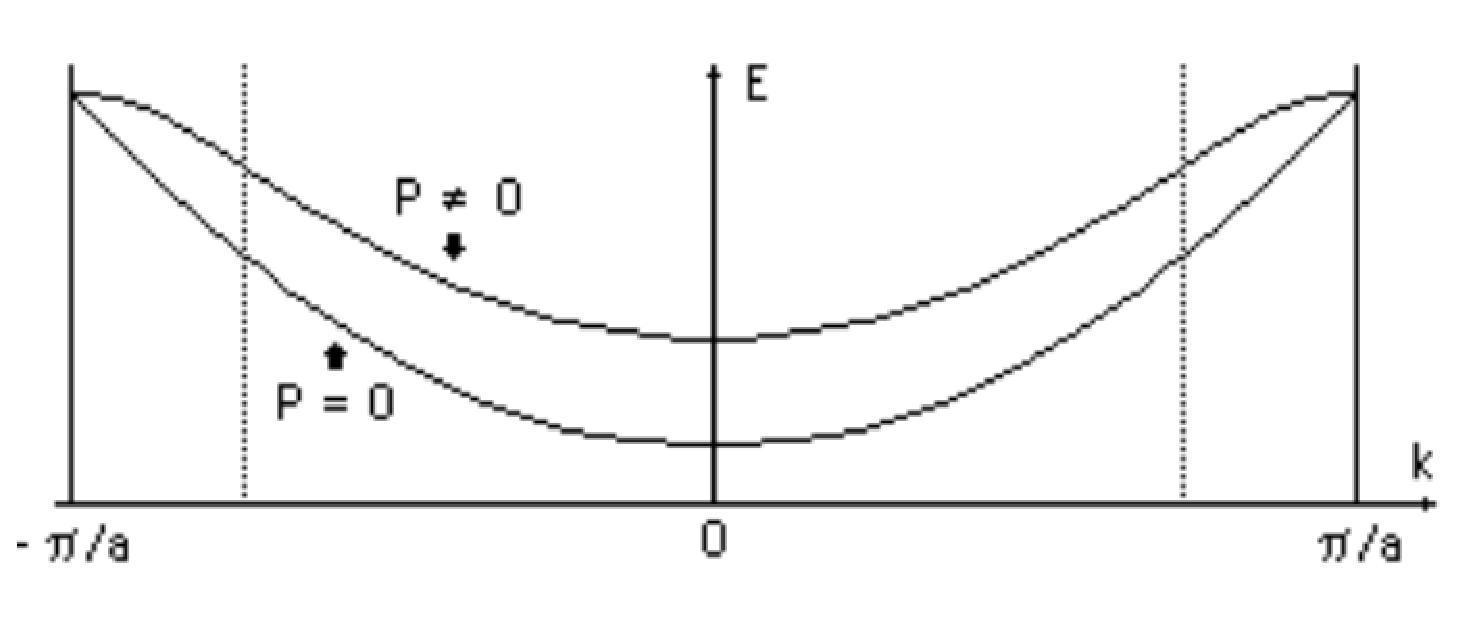
\includegraphics[scale=0.4]{somer.eps} \\
Si on prend l'autre cas extrême ($P\rightarrow \infty$) les barrière de potentiel ne peuvent plus être traversées, même par effet tunnel, et l'on obtient des niveaux d'énergie discrets. C'est en fait le modèle de l'électron dans un puits de potentiel infini. \\
%Finalement, si on enlève l'hypothèse d'un cristal infini, et qu'on applique les conditions cycliques de Born-von Karman, on obtient que les bandes d'énergie deviennent alors discrètes. Les conditions de Born-von Karman consistent à dire que le cristal infini est constitué d'un nombre infini de cristaux finis identiques.
Pour généraliser à un cristal de longueur finie $L$, on considère la juxtaposition d'une infinité de cristaux identiques. On peut alors utiliser les résultats pour une cristal infini en ajoutant une condition (condition cyclique de Born-von Karman) : $\Psi(x+L,t) = \Psi(x,t)$. On obtient alors une quantification de $k$.
\subsection{Vitesse de groupe}
Pour connaître la vitesse des électrons dans le cristal, il faut prendre la vitesse de groupe du paquet d'onde qui les représente (formé par la somme des fonctions d'onde de chaque électron); Celle-ci est donnée par :
\begin{equation}
v_g=\frac{1}{\hbar}grad(E(k))
\end{equation}
Il en découle que la vitesse est une fonction impaire  ($v_g(-k)=-v_g(k)$), ce qui signifie aussi que la vitesse de phase en zéro est nulle. %La vitesse des électrons est également nulle au bord de la zone de Brillouin, ce qui est dû à la réflexion des électrons sur les plan de Brag (qui définissent la limite de la zone de Brillouin; ils sont définis comme les plans médiateurs des vecteurs de base du réseau réciproque). 
Finalement on remarquera que le modèle de Sommerfeld n'est valable que pour des petits vecteurs d'onde. 
\\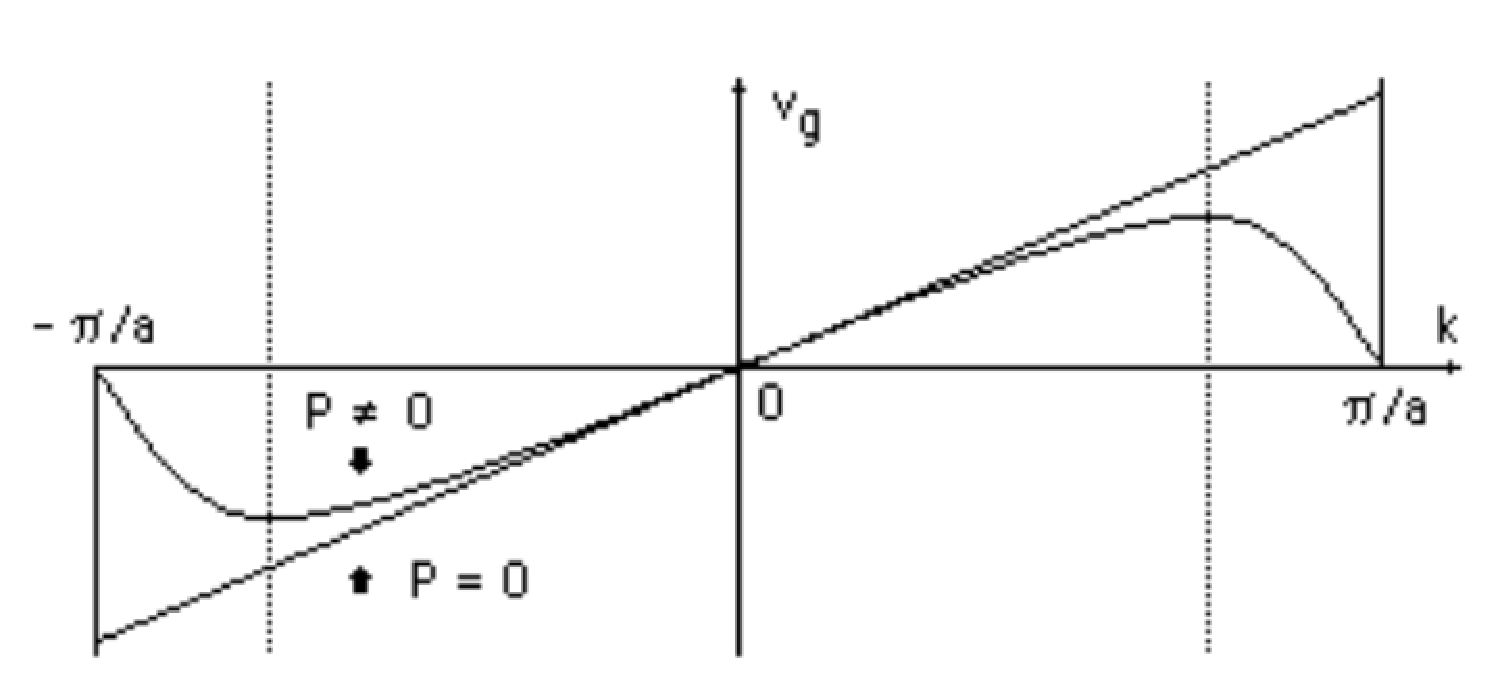
\includegraphics[scale=0.4]{vitesse.eps} \\
Remarque : la vitesse des trous est la même que la vitesse des électrons.
\subsection{Masse effective}
La masse effective d'un électron est la masse que devrait avoir cet électron dans le vide pour réagir à des forces extérieures de la même façon que dans le cristal. La masse effective contient l'effet global du potentiel cristallin sur l'électron. On suppose que les forces extérieures restent faibles par rapport aux force cristallines et que les potentiels qui en dérivent varient lentement. Il en découle que la masse effective est inversement proportionnelle au laplacien de l'énergie :
\begin{equation}
\frac{1}{m^*}=\frac{1}{\hbar^2} \triangle E(k)
\end{equation}
La masse effective $m^*$ n'est donc plus nécessairement scalaire, ce qui entraine que l'accélération n'est pas nécessairement colinéaire à la force appliquée. On remarque également que la masse effective est négative quand le gradient de la vitesse est négatif, qu'elle est nulle au niveau aux bord de la zone de Brillouin et égale à la masse de l'électron pour les vecteurs d'onde nuls. A nouveau, le modèle de Sommerfeld n'est valable que pour de faibles valeurs du vecteur d'onde (ou plus précisément, près du minimum de la bande d'énergie considérée).
\\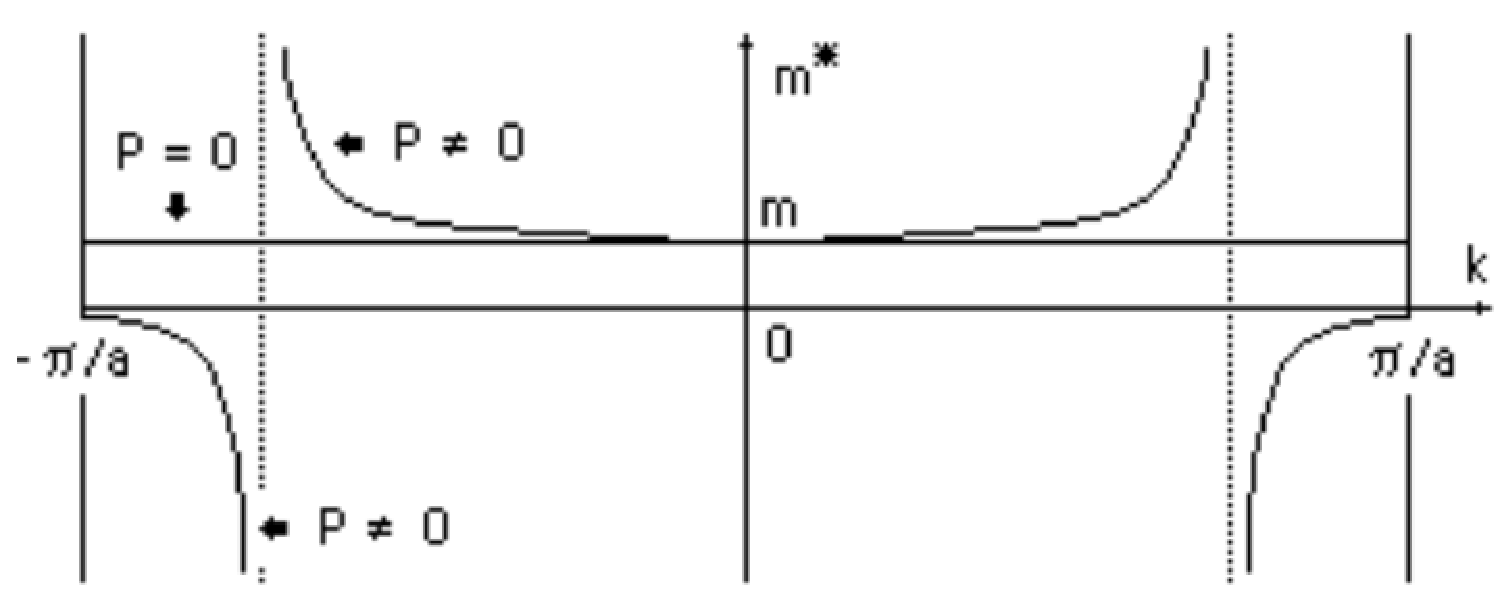
\includegraphics[scale=0.4]{masse.eps}
\subsection{Contribution au courant d'une bande pleine d'électrons}
Considérons dans un premier temps un seul électron de charge $-q$ avec une vitesse $v_g$ dans un cristal de volume $V$. La contribution à la densité de courant de cet électron est, avec V le volume :
\begin{equation}
\mathbf{J}=-\frac{q\mathbf v_g}{V}
\end{equation}
Cet électron appartient à une bande d'énergie $E(k)$, la densité (de vecteur d'onde dans une bande d'énergie) d'états permis dans un cristal de volume $V$ est donnée par $V/8\pi^3$. La fonction de distribution (des électrons dans la bande) de ces états permis, notée $f(k)$, est égale à la fonction de Fermi-Dirac si on est à l'équilibre thermodynamique. Le nombre d'électrons qui occupent la bande est donc donné par :
\begin{equation}
2\frac{V}{8\pi ^3} f(k)
\end{equation}
Le facteur 2 vient du fait que l'on peut avoir 2 électrons de spin opposé sur le même niveau d'énergie (principe d'exclusion de Pauli). L'ensemble de tous les électrons de la bande est donc donné par l'intégrale de la densité de courant sur toute la zone de Brillouin.

\begin{equation}
\mathbf{J} =\int_{ZB}\frac{V}{4\pi^3}f(\mathbf{k})\frac{-q\mathbf v_g}{V}=\frac{-q}{4\pi^3}\int_{ZB}f(\mathbf{k}) \mathbf{v_g}(\mathbf{k}) \ d\mathbf{k}
\end{equation}
Si la bande est complètement remplie d'électrons, on a $f(k)=1$ pour tout vecteur k de la bande d'énergie,et on sait que la vitesse de groupe $v_g$ est une fonction impaire de $k$, l'intégrale sur une période de celle-ci sera donc nulle :
\begin{equation}
\mathbf{J}=0.
\end{equation}
La contribution au courant d'une bande d'énergie complètement remplie est donc nulle !
%------------------------------
\section{Question 2}
Décrire la relation (E, k), ainsi que la variation de vitesse des porteurs et leur masse
effective, en fonction de k dans un cristal unidimensionnel infini. Indiquez les zones de
masse effective positive et négative pour les électrons.
\\
\hbox{\raisebox{0.4em}{\vrule depth 0pt height 0.4pt width 6cm}}
\\
Voir question précédente.
%----------------------------------
\section{Question 3}
Pourquoi la notion de trou a-t-elle été introduite et en quoi est elle utile pour décrire la
conduction dans un semi-conducteur? Quels sont les mécanismes qui induisent le transport
de charge ? Quelle relation permet de l'exprimer ?
\\
\hbox{\raisebox{0.4em}{\vrule depth 0pt height 0.4pt width 6cm}}
\\
On sait qu'une bande remplie d'électrons ne conduit pas le courant. Par contre, si on retire un électron de la cette bande d'énergie, tout est comme si on on avait une seule particule de charge opposée à celle de l'électron dans la bande. En effet :
\begin{equation}
\mathbf{J}=0-\frac{-q\mathbf{v_g}(\mathbf{k})}{V}=\frac{+q\mathbf{v_g}(\mathbf{k})}{V}
\end{equation}
Cette nouvelle particule a donc une charge opposée à celle de l'électron (donc +q), sa vitesse $v_g$ est celle de l'électron manquant et sa masse effective est par définition opposée à celle de l'électron manquant. Les trous positifs sont utilisés pour caractériser une bande d'énergie qui est presque remplie d'électrons, on travaille donc au niveau du maximum d'énergie d'une bande. Le manque de plusieurs électrons s'exprime comme si on avait plusieurs trous. La fonction de distribution vaut donc $1-f(k)$.
\paragraph*{}
Dans un cristal parfait, sans aucune perturbation extérieure, les charges restent fixes. Seulement, aucun cristal n'est parfait, car il peut contenir des défauts tels que des lacunes, des dislocations, des joints de grain... auxquels s'ajoute l'agitation thermique qui génère des phonons. Il y aura dès lors interactions (des collisions) entre les charges, les différentes impuretés ou encore avec les phonons, avec comme résultat un mouvement aléatoire des charges. En l'absence de force extérieure, celui-ci sera nul en moyenne ; mais si on applique un champ électrique, on observe une tendance à dériver dans la direction opposée. de plus, si il existe un gradient de porteurs, ceux-ci vont diffuser afin de rétablir l'équilibre (première loi de Fick).
La densité de courant (qui est une mesure du mouvement des charges) dans un matériau est donc donnée par la somme des deux contributions :
\begin{equation}
\begin{array}{c}
J_n=q[n\mu_nE+D_n \frac{\partial n}{\partial x }]
\\ 
J_p=q[p\mu_pE-D_p \frac{\partial p}{\partial x }]
\end{array} 
\end{equation}
avec n pour les électrons et p pour les trous. Le terme $qn\mu_nE$ représente le courant de dérive avec $\mu_n$ la mobilité des électrons et le terme $D_n \frac{\partial n}{\partial x }$ le courant de diffusion avec $D_n$ le coefficient de diffusion des électrons. (On voit que s'il existe un gradient de porteurs dans un matériau, un champ électrique interne va apparaître et rétablir l'équilibre) %En l'absence de champ $E$ extérieur et d'un gradient de charges ($\frac{\partial n}{\partial x }=0$), le courant J est nul. S'il existe un gradient de charges à l'équilibre (les charges à l'équilibre sont $n_0$ et $p_0$), on a J=0 (par définition de l'équilibre) et donc :
%\begin{equation}
%\begin{array}{c}
%n\mu_n E=-D_n \frac{\partial n}{\partial x }
%\\ 
%p\mu_pE = D_p \frac{\partial p}{\partial x }
%\end{array} 
%\end{equation}
%Le courant de dérive compense donc le courant de diffusion. Maintenant, si un champ électrique extérieur est appliqué, on rompt l'équilibre et J devient non nul. 

Le courant total vaut la somme des courants de trous et des courants d'électrons :
\begin{equation}
J_{tot}=J_n+J_p+\epsilon \frac{\partial E}{\partial t }
\end{equation}
avec le dernier terme le courant de déplacement dans le cas d'une variation temporelle de champ électrique. 
Le coefficient de diffusion est donné par les relations d'Einstein :
\begin{equation}
\begin{array}{c c}
D_n = \mu_n \frac{kT}{q} & D_p=\mu_p \frac{kT}{q}
\end{array}
\end{equation}
%Finalement, il faut faire attention que la concentration de porteurs n et p peut varier pour 2 raisons :
%\begin{enumerate}
%\item Les forces extérieures engendrent une divergence du courant et donc une modification locale de la densité de charge.
%\item Il peut y avoir des phénomènes de recombinaison (U) (disparition des porteurs) ou de génération (G) (apparition de porteurs) de porteurs dans une bande considérée.
%\end{enumerate}
%On obtient donc :
%\begin{equation}
%\begin{array}{c}
%\frac{\partial n}{\partial t }=\frac{1}{q} div(J_n)+G_n-U_n
%\\ 
%\frac{\partial p}{\partial t }=-\frac{1}{q} div(J_p)+G_p-U_p
%\end{array} 
%\end{equation}

%-----------------------------------
\section{Question 4}
Comment déterminer le niveau de Fermi d’un métal pur ?  Donnez l'ordre de grandeur pour l'energie qui separe $E_F$ du bas de la bande de conduction\\
\hbox{\raisebox{0.4em}{\vrule depth 0pt height 0.4pt width 6cm}}
\\
Dans un métal, la bande de conduction est partiellement remplie d'électrons, le niveau de Fermi est donc dans la bande de conduction. Le nombre d'électrons dans cette bande, à l'équilibre, est donné par :
\begin{equation}
n=2\int_{E_c}^{E_{cM}} f(E)N_c(E)dE 
\end{equation} 
Avec $f(E)$ la fonction de distribution des états et $N_c$ le nombre d'états permis. La fonction de distribution est, dans ce cas, la fonction de Fermi-Dirac qui ne peut pas être approximée par Maxwell-Boltzmann car on est dans la bande de conduction. On ne sait donc pas résoudre analytiquement l'équation obtenue. Une solution est de remarquer que le produit $N(E).f(E)$ devient très vite négligeable quand $E>\mu$. On peut donc intégrer de  $E-E_c = 0$ à $\infty$ et utiliser une bonne approximation (dont le résultat des connu) de l'intégrale de la fonction de F-D.%faire un développement en séries de la fonction à intégrer, de tronquer cette série à l'ordre qui nous intéresse (en l'occurrence l'ordre 1) et d'intégrer celle-ci.
Connaissant le nombre d'électrons libres dans le métal (en général de $10^{22}$ à $10^{23}$), on peut alors calculer l'énergie de Fermi $(E_c-\mu)$. Après différents développement, on arrive au résultat suivant pour $0K$ :
\begin{equation}
(\mu -E_c)_0=\frac{h^2}{8m_c} (\frac{3n}{\pi})^{2/3}
\end{equation}
Pour $T \neq 0$ :
\begin{equation}
\frac{\mu -E_c}{(\mu - E_c)_0} = \frac{1}{\left[ 1 + \frac{\pi^2}{8} \left( \frac{kT}{\mu - E_c} \right)^2 \right]^{2/3}}
\end{equation}
Cette énergie de Fermi ($\mu -E_c$) d'un métal est de l'ordre de 5~eV. A 300k, $kT = 0.025 eV$. Si $kT \ll (\mu - E_c)$, on voit que $(\mu - E_c)$ diffère très peu de $(\mu - E_c)_0$ . \\

En faisant un développement en série, on arrive à l'approximation suivante qui montre que l'énergie de Fermi d'un métal reste pratiquement constante en fonction de la température:
$$ \mu - E_c = (\mu - E_c)_0 \left[ 1 - \frac{\pi^2}{12} \left( \frac{kT}{(\mu - E_c)_0}\right)^2 \right]$$

\subsection{Effet Schottky (supplément)}
Soit un métal dans le vide. Le travail qu'il faut pour extraire un électron du métal est $W=-\mu_0$ avec $\mu_0$ le niveau de Fermi. On peut ainsi calculer l'énergie du bas de la bande de conduction à l'aide de l'énergie de Fermi calculée précédemment. \\
Si on applique un champ électrique, l'énergie potentielle de l'électron possède un maximum unique $x_0$. En ce point, l'énergie d'extraction va être diminuée d'une valeur $\Delta W$ proportionnelle au radical de champ électrique appliqué. C'est ce qu'on nomme l'effet Schottky.\\
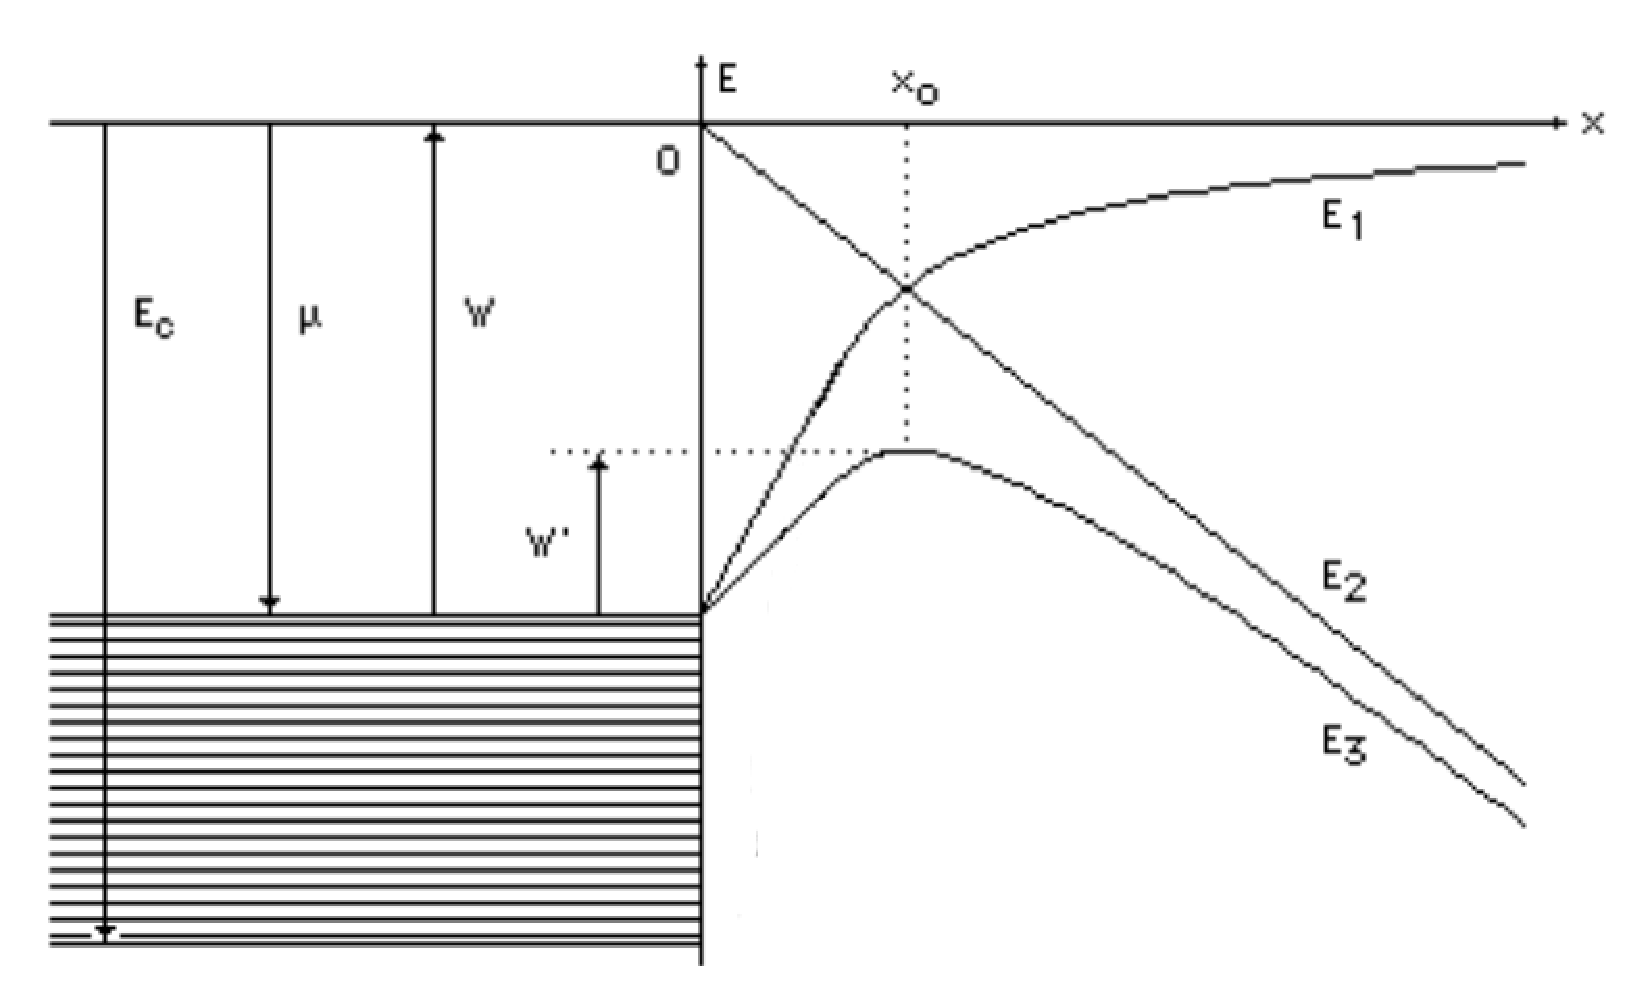
\includegraphics[scale=0.4]{schottky.eps}\\
Avec $w$ le travail de sortie sans champ électrique, $w'$ le travail avec un champ électrique et $E_1$ l'énergie de rappel de l'électron (énergie de la barrière de potentiel) :
\begin{equation}
E_1=-\frac{q^2}{4\pi\epsilon_0 (2x)^2}=-\frac{q^2}{16\pi\epsilon_0 x}
\end{equation}
$E_2$ est l'énergie potentielle de l'électron dans le champ appliqué ($E_2=-qEx$) et $E_3$ la somme de ces deux énergies. Le maximum d'énergie est en $x_0$ pour lequel l'énergie d'extraction n'est plus que de $w'$ au lieu de $w$ 
%--------------------------
\section{Question 5}
Décrire les différents types d'impuretés présentes, volontairement ou non, dans un semi-conducteur et décrire leurs effets  sur les propriétés et la densité des porteurs de charge.
\\
\hbox{\raisebox{0.4em}{\vrule depth 0pt height 0.4pt width 6cm}}
\\
Les différents types d'impuretés sont:
\begin{enumerate}
\item Les lacunes (sites dépourvus d'atomes)
\item Une lacune et un atome en position interstitielle (paire de Frenkel)
\item Les dislocations (défauts complexes)
\item Atomes différents présents dans le cristal (non pur)
\end{enumerate}
Ajouter des atomes différents dans le cristal dans une quantité connue peut apporter des propriétés électriques au matériaux.  Un exemple est l'ajout de Bore ou Phosphore dans du silicium. \\Dans des concentrations normales de défauts et sous un dopage normal, il y a un maintient des bandes d'énergie permises et interdites du cristal intrinsèque et l'introduction de nouveaux niveaux d'énergie localisés à l'endroit de l'imperfection.
\begin{enumerate}
\item Si le niveau d'énergie se situe dans une bande d'énergie permise, la densité d'état de celle-ci augmente légèrement, mais les propriétés ne varient presque pas.
\item Si les niveaux se trouvent dans une bande d'énergie interdite, on a alors une forte modification des propriétés électroniques.
\end{enumerate}
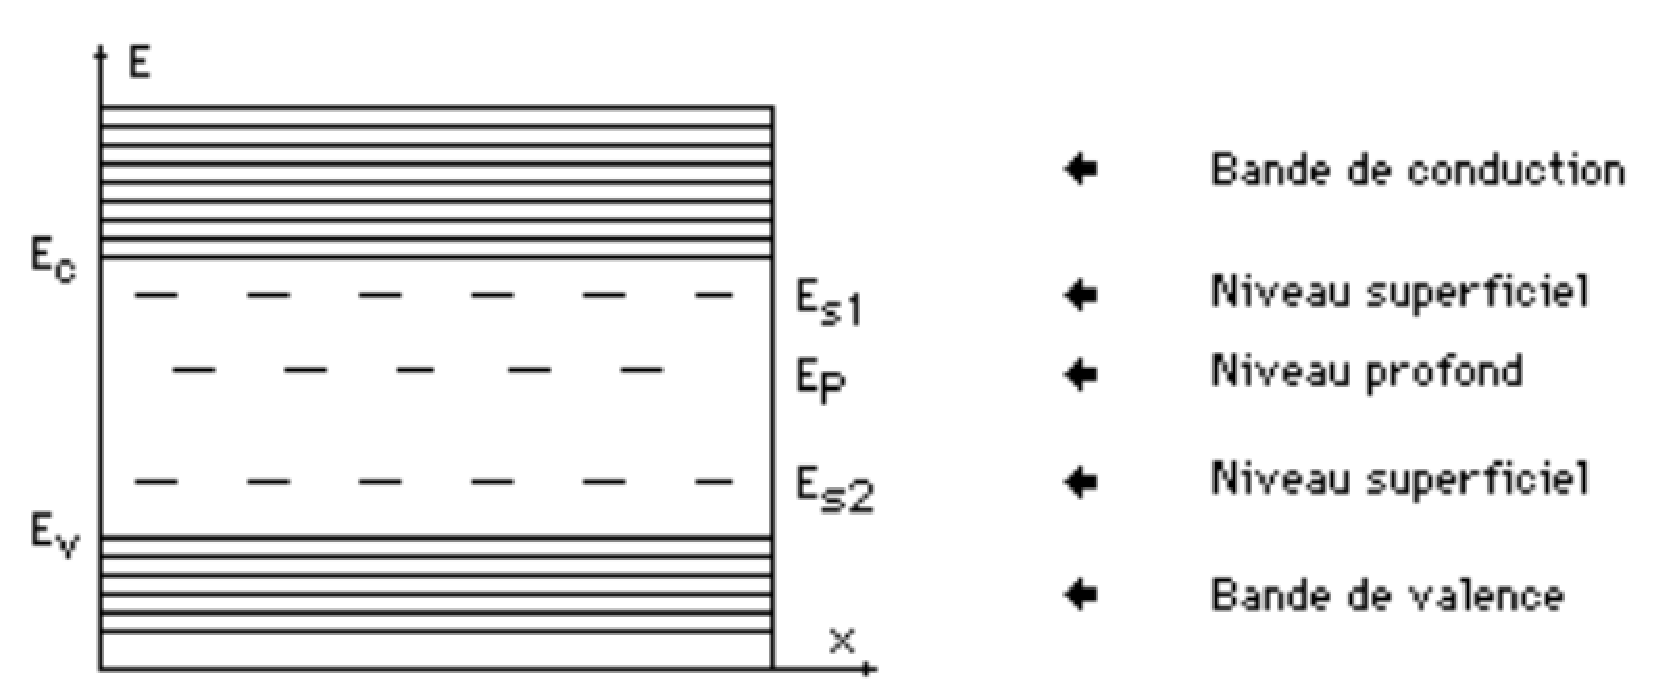
\includegraphics[scale=0.3]{niv.eps} \\
On peut distinguer deux type de niveaux, les niveaux superficiels qui se trouvent proches d'une bande d'énergie, et les niveaux profonds qui se trouvent proches du centre de la bande interdite. 
\begin{description}
\item[Les niveaux superficiels] interagissent fortement avec les électrons (niveaux donneurs) et les trous (niveaux accepteurs) et favorisent ainsi énormément la conductivité électronique.
\item[Les niveaux profonds: ] localisés près du milieu de la bande interdite, ils interagissent simultanément avec les deux bandes permises et, par ce fait, influencent le transfert de porteurs entre bandes permises (phénomènes de recombinaison et génération de porteurs). 
\end{description}

Les niveaux donneurs sont dus à des atomes ayant un atome de plus que le semi-conducteur à doper (dans le cas du silicium, pentavalents comme le Phosphore). Cet électron va occuper le niveau extrinsèque tant qu'il n'est pas ionisé, auquel cas il passera dans la bande de conduction, généralement proche. Des électrons seront donc "donnés" pour améliorer la conduction.
\begin{equation}
P+\Delta E=P^+ + (-q)
\end{equation} 
Si la concentration n d'électrons dans la bande de conduction est dominante par rapport à la concentration en trous p dans la bande de valence, le semi-conducteur est de type N. On observe que l'ajout d'atomes donneurs a pour effet de rapprocher de niveau de Fermi vers le haut de la bande interdite.
\\ 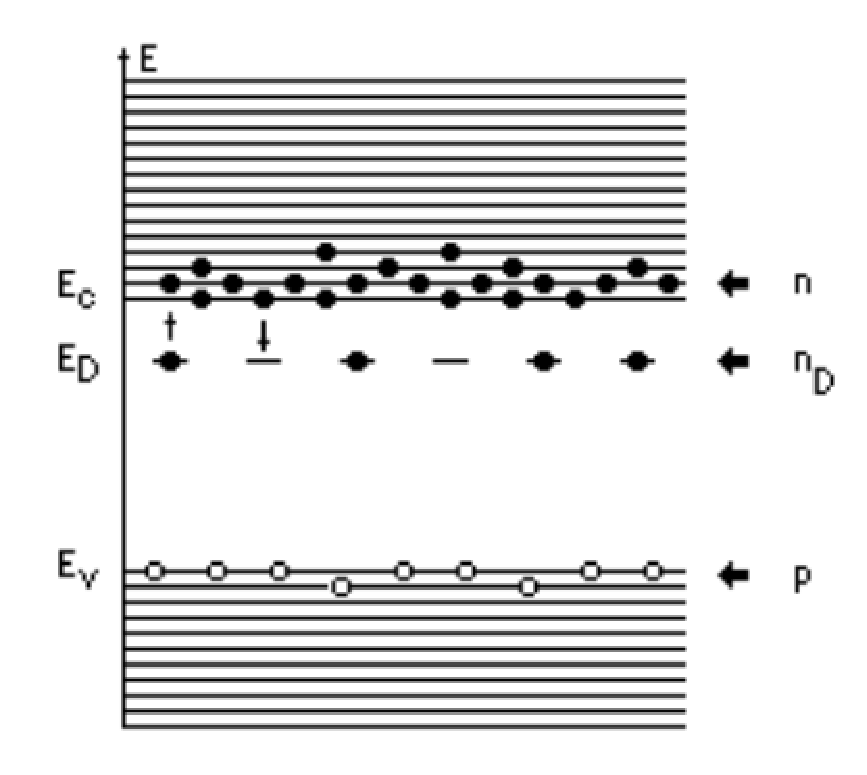
\includegraphics[scale=0.3]{doner.eps} \\
Les niveaux accepteurs sont dus à des atome trivalents comme le Bore (B), qui laissera une liaison vide au silicium. Ces niveaux peuvent donc recevoir des électrons, ce qui permet de former des trous dans la bande de valence, souvent proche, a et ainsi augmenter le courant de trous.
\begin{equation}
B+\Delta E=B^- + (+q)
\end{equation} 
Si la concentration p est plus grande que n, on a un semi-conducteur de type P. Le niveau de Fermi est dans ce cas plus bas que le niveau de Fermi intrinsèque.
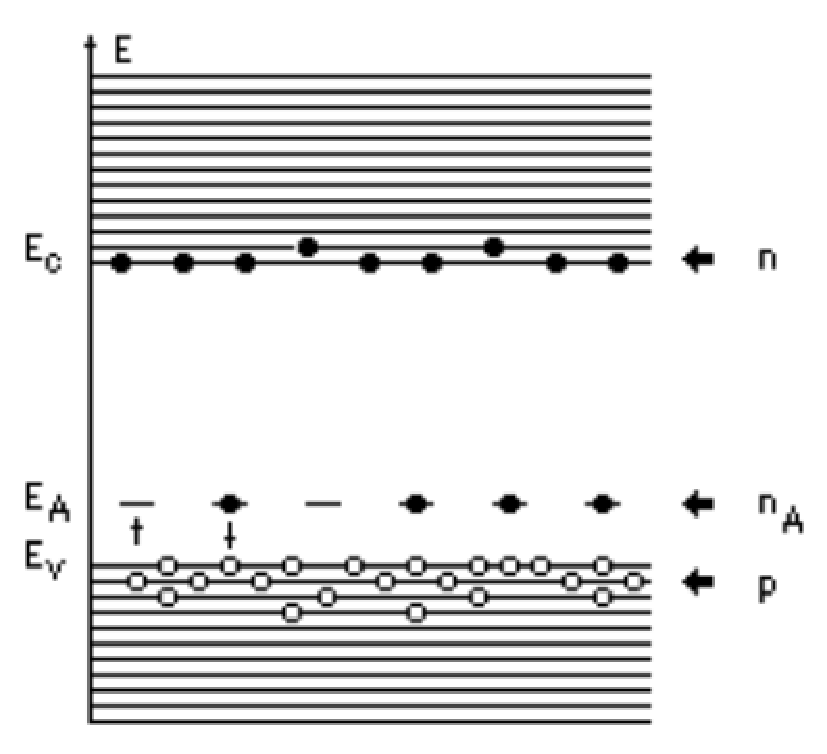
\includegraphics[scale=0.3]{accepteur.eps}\\
Si un atome crée plusieurs niveaux d'énergie dans la bande interdite, on parle de centre multivalent.

L'ajout d'impuretés permet donc d'augmenter la densité d'un type de porteurs, dans une proportion donnée par l'équation de neutralité électrique:
\begin{equation}
p+N_D^+=n+N_A^-
\end{equation}
avec $N_D^+$ et $N_A^-$ les densités de centres ionisés. À température ambiante, on a généralement : $N_D^+ \simeq N_D$ et $N_A^- \simeq N_A$, c'est-à-dire que la plupart des centres sont ionisés. 

Cependant, on peut prouver que dans tous les cas, le produit $np$ reste constant et vaut le carré la concentration intrinsèque $n_i$.\\

\subsubsection{Supplément :}

Le nombre de centres ionisés est donné par :
$$
N_D^+=\frac{N_D}{1+2~exp\left(\frac{E_F-E_D}{kT}\right)}
$$
$$
N_A^-=\frac{N_A}{1+2~exp\left(\frac{E_A-E_F}{kT}\right)}
$$
Avec $N_D^+$ et $N_A^-$ les densités de donneurs/accepteurs ionisés, $E_F$ le niveau de Fermi et $E_D$/$E_A$ le niveau d'énergie des centres donneurs/accepteurs. On constate généralement qu'a température ambiante (300K), la plupart des centres donneurs/accepteurs sont ionisés. Même si on ajoute des impuretés, la neutralité électrique est toujours conservée :
\begin{equation}
p+N_D^+=n+N_A^-
\end{equation}
Outre les porteurs de charges dus aux centres donneurs et accepteurs, il y a également des porteurs générés directement entre les 2 bandes d'énergie, on a dès lors génération simultanée d'électrons et de trous. Dans un cristal sans impureté, on a donc que le nombre d'électrons est égal au nombre de trous, cette concentration de porteurs est appelée concentration intrinsèque $n_i$ et dépend de la température et de la largeur de la bande interdite. On a donc :
\begin{equation}
n_i^2=np
\end{equation}
Cette formule reste valable en présence de centres donneurs et accepteurs. Finalement, dans un semi-conducteur non dégénéré, le nombre de porteurs est donné par :
\begin{equation}
\begin{array}{c}
n=n_i~exp\left(\frac{E_f-E_i}{kT} \right)\\
p=n_i~exp\left(\frac{E_i-E_f}{kT} \right)
\end{array} 
\end{equation}
Avec $ n_i$ la concentration intrinsèque, $E_f$ le niveau de Fermi et $E_i$ le niveau intrinsèque d'un cristal parfait (qui se trouve approximativement au milieu de la bande interdite).
%-------------------------
\section{Question 6}
Dans quelles limites la fonction de distribution de Maxwell-Boltzmann constitue-t-elle une bonne approximation pour les électrons dans le silicium ?
\\
\hbox{\raisebox{0.4em}{\vrule depth 0pt height 0.4pt width 6cm}}
\\
\begin{equation}
\begin{array}{c| c}
\mbox{Fermi-Dirac} &\mbox{ Maxwell-Boltzman} \\ 
\hline \\
f(E)=\frac{1}{1+exp\left(\frac{E-\mu}{kt}\right) } & f(E)=\frac{1}{exp\left( \frac{E-\mu}{kt} \right) }\\ 
\end{array} 
\end{equation}
On Approxime FD par MB quand l'exponentielle devient beaucoup plus grande que 1, et que l'on peut donc négliger ce facteur. Cette approximation nécessite dès lors que $(E-\mu)$ soit grand. On obtient une erreur inférieur à 5\% si on considère qu'il faut que $E-\mu>3kT$ (avec $kT=0.025eV$ à $300K$). Cette condition est par définition la condition pour avoir un semi-conducteur non-dégénéré. C'est à dire qu'il faut que le niveau d'énergie de Fermi soit à plus de $3kT$ d'une bande d'énergie (en l'occurrence, la bande de conduction et la bande de valence). Dans la plupart des cas, l'approximation de Maxwell-Boltzmann peut être utilisée car le semiconducteur est dégénéré.
%-----------------------
\section*{Question 6.2}
Définissez à l'aide de la relation analytique ce que sont : un semi-conducteur dégénéré, non-dégénéré, intrinsèque, extrinsèque. décrivez comment la température peut faire passer un semi- conducteur d'une catégorie vers l'autre. \\
\hbox{\raisebox{0.4em}{\vrule depth 0pt height 0.4pt width 6cm}} \\
\begin{description}
\item [Un semiconducteur non dégénéré] est un semiconducteur qui possède son niveau de Fermi dans la bande interdite.  On a que $ | E_c-E_f | > 3kT$ et $ | E_v-E_f | > 3kT$, ce qui permet d'utiliser l'approximation de Maxwell-Boltzmann.
\item [Un semiconducteur dégénéré] ne respecte pas cette relation.
\item[Un semiconducteur est dit intrinsèque] si les porteurs présents ne proviennent que de l'excitation thermique. La condition de neutralité électrique impose que $n = p = n_i$.  Le niveau de Fermi se trouve approximativement au milieu de la bande interdite et s'appelle le niveau intrinsèque $E_i$.
\item[Un semiconducteur extrinsèque] est un semiconducteur dopé N ou P. La densité de dopant est supérieure à la densité intrinsèque $n_i$. L'équilibre électronique reste conservé et on a toujours $np = n_i^2$.
\end{description}

En augmentant la température, on peut faire passer le semiconducteur d'un état extrinsèque vers un état intrinsèque. Si les droites se croisent au-dessus du niveau de dopage, alors le semiconducteur est redevenu intrinsèque, comme illustré à la figure \ref{intrinseque}.
\begin{figure}[h!] %Here,Top,Bottom,Page
\begin{center}
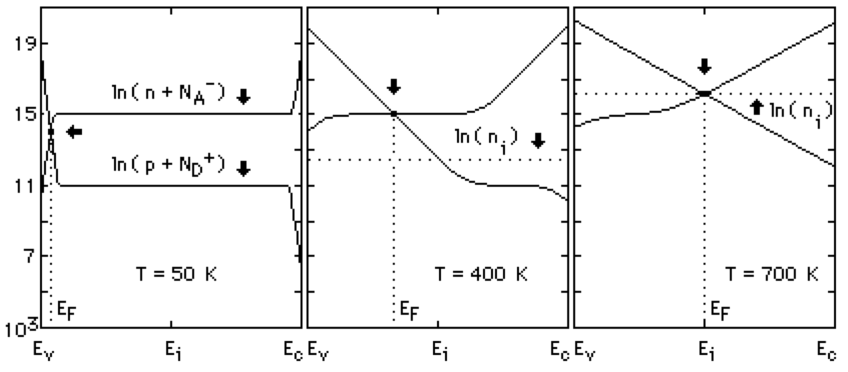
\includegraphics[height=6cm]{intrinseque}
\caption{}
\label{intrinseque}
\end{center}
\end{figure} 
%-----------------------
\section{Question 7}
Expliquez la différence entre phonons optiques et phonons acoustiques : origine physique, relation entre énergie et vecteur d'onde,... Donnez la dépendance en température de la mobilité des porteurs dans le silicium en fonction du dopage et identifiez la contribution des phonons.
\\
\hbox{\raisebox{0.4em}{\vrule depth 0pt height 0.4pt width 6cm}}
\\
On considère une chaine  linaire d'atomes vibrant autours d'une position initiale. Si on considère un cristal infini, on peut utiliser le théorème de Bloch (le réseau cristallin est périodique) et trouver la relation de dispersion qui lie la pulsation $\omega$ au vecteur d'onde $q$:
\begin{equation}
\omega(q) =\omega_c \left| sin\left(\frac{qa}{2} \right) \right|
\end{equation}
Avec $\omega_c$ la pulsation de coupure (pulsation maximale). La pulsation est une fonction périodique, qui a la périodicité du réseau réciproque; on peut donc limiter l'étude de celle-ci à la première zone de Brillouin. On remarque également que la pulsation est une fonction paire de vecteur d'onde ($\omega(-q)=\omega(q)$).
\\ 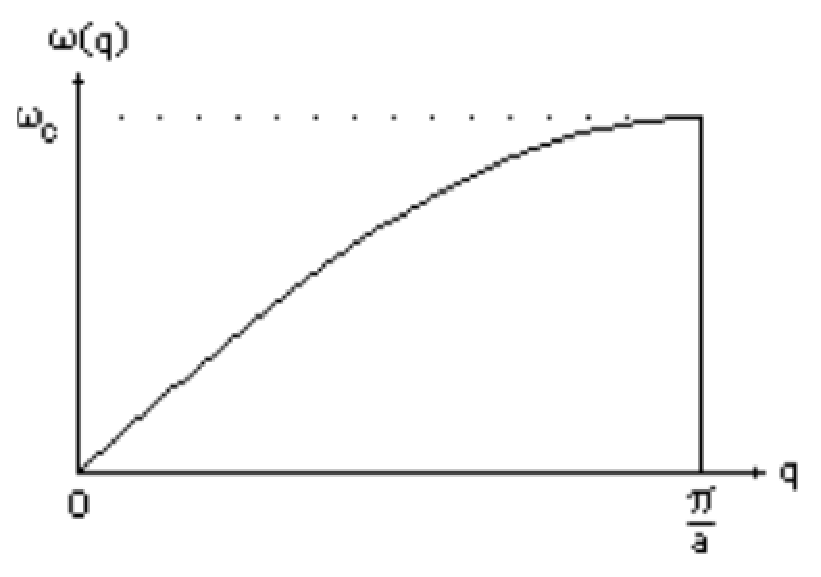
\includegraphics[scale=0.4]{wdis.eps} \\
Si on repasse dans le cadre d'un cristal fini, il faut appliquer les conditions cycliques de Born-von Karman. Il en résulte une discrétisation de la fonction de dispersion. La solution de l'équation de Schrodinger pour la vibration d'une chaine mono-atomique montre que l'énergie associée à la vibration du cristal est quantifiée de la manière suivante :
\begin{equation}
E=(n+\frac{1}{2})\hbar \omega(q)
\end{equation}
Il existe donc une énergie de point zéro : quand il n'y a plus aucune vibration, l'énergie est toujours non nulle. Comme cette énergie est quantifiée, on peut exprimer celle-ci comme une somme de quanta d'énergie (à l'énergie du point zéro près). Ces quanta sont appelés phonons. L'énergie totale de vibration E est donc la somme des énergies de N phonon d'énergie $ \hbar \omega(q) $ auxquels s'ajoute une énergie du point zéro. 
Si on étudie une chaine di-atomique, qui est donc constituée de 2 types d'atomes de masse différente, on observe l'ouverture d'une bande interdite dans la relation de dispersion de $\omega$.
\\ 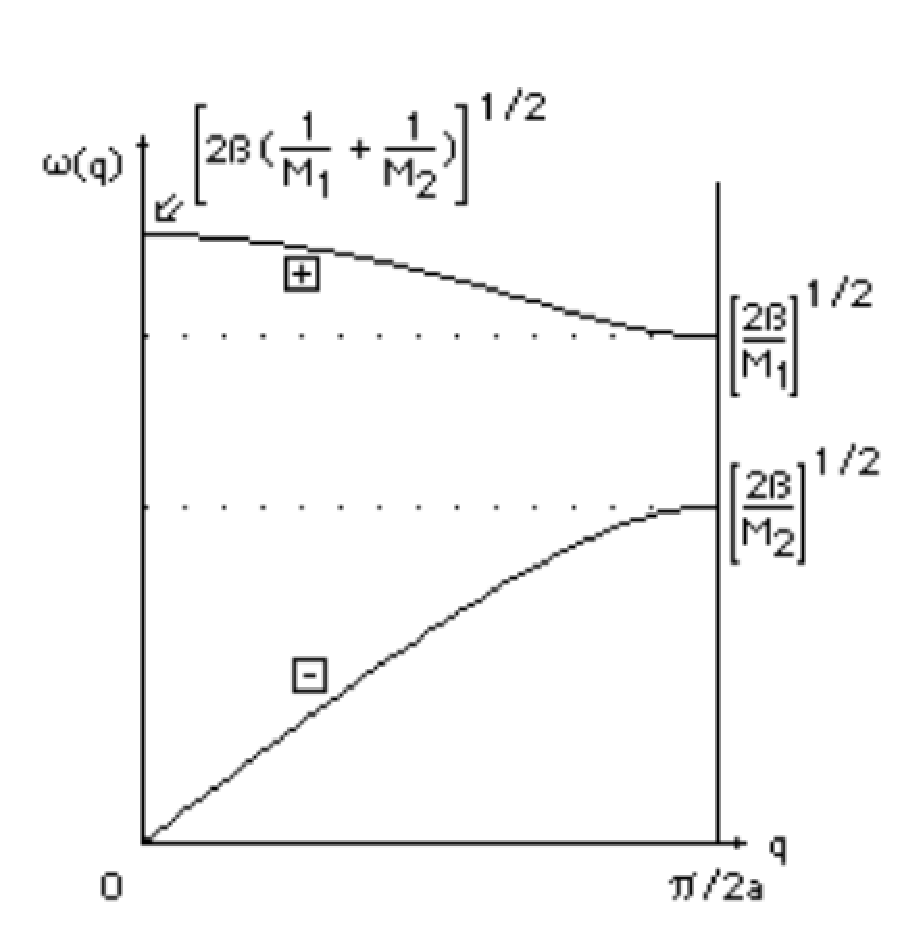
\includegraphics[scale=0.4]{wdis2.eps} \\
Il existe donc plusieurs modes de vibrations. Les phonons acoustiques correspondent au mode basse fréquence ($\omega_-$) alors que les phonons optiques correspondent au mode haute fréquence ($\omega_+$). Les modes basse et haute fréquence sont séparés par un gap, une bande interdite, qui est fonction de la différence de masse entre les 2 atomes de la chaine diatomique considérée (si la masse est égale, il n'y a pas de bande interdite).Les propriété de le fonction de distribution ne changent pas et l'on peut donc étudier la fonction dans la première zone de Brillouin (remarquons que la fonction est également symétrique ).\\
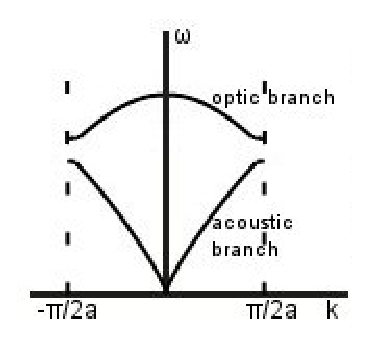
\includegraphics[scale=1]{diatomic-dispersion-relation1.eps} 
\paragraph*{}
La mobilité des porteurs est influencée par deux phénomènes différents. D'un coté, on a une influence des collisions entre les porteurs et le réseau, c'est à dire majoritairement avec des phonons créés par l'agitation thermique. On a alors :
\begin{equation}
\mu _r=\frac{A}{T^{3/2}}
\end{equation}
D'un autre coté, La mobilité est inversement proportionnelle à la concentration des impuretés chargées $N_i$ qui vont ralentir également les porteurs de charge.
\begin{equation}
\mu _i=\frac{B T^{3/2}}{N_i}
\end{equation}
La mobilité total est alors obtenue par combinaison de $\mu _i$ et $\mu _r$ :
\begin{equation}
\frac{1}{\mu}=\frac{1}{\mu _i}+\frac{1}{\mu _r}
\end{equation}
\\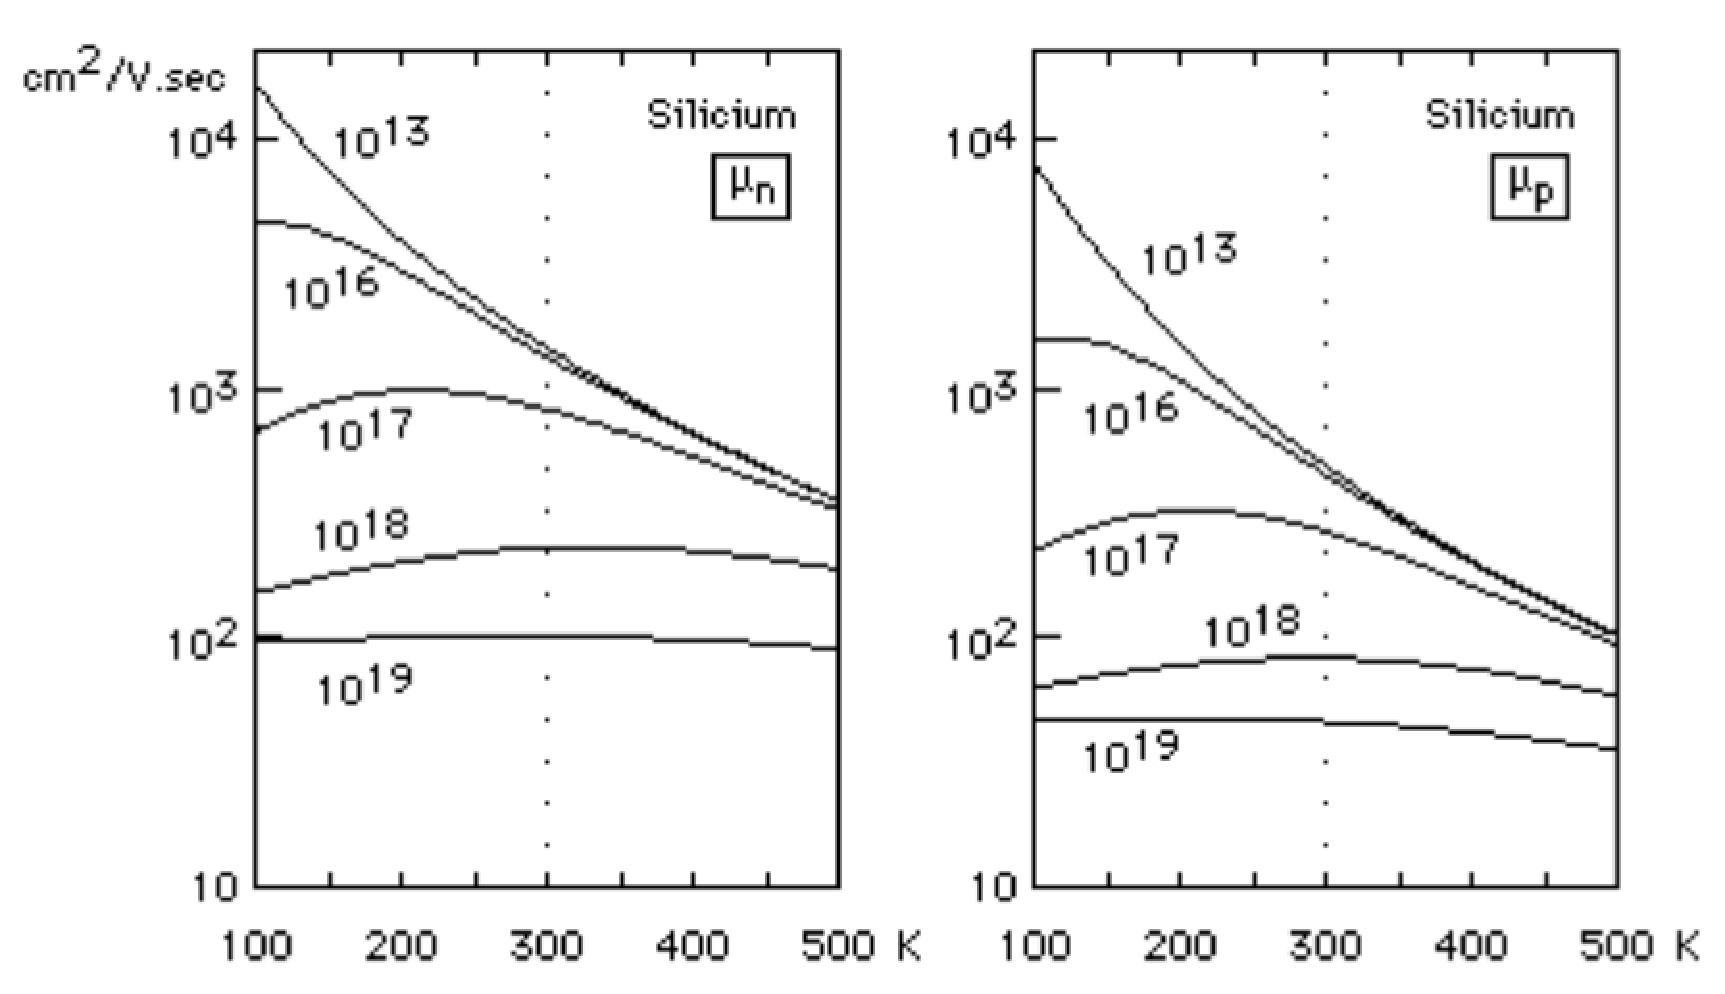
\includegraphics[scale=0.3]{mut.eps} 
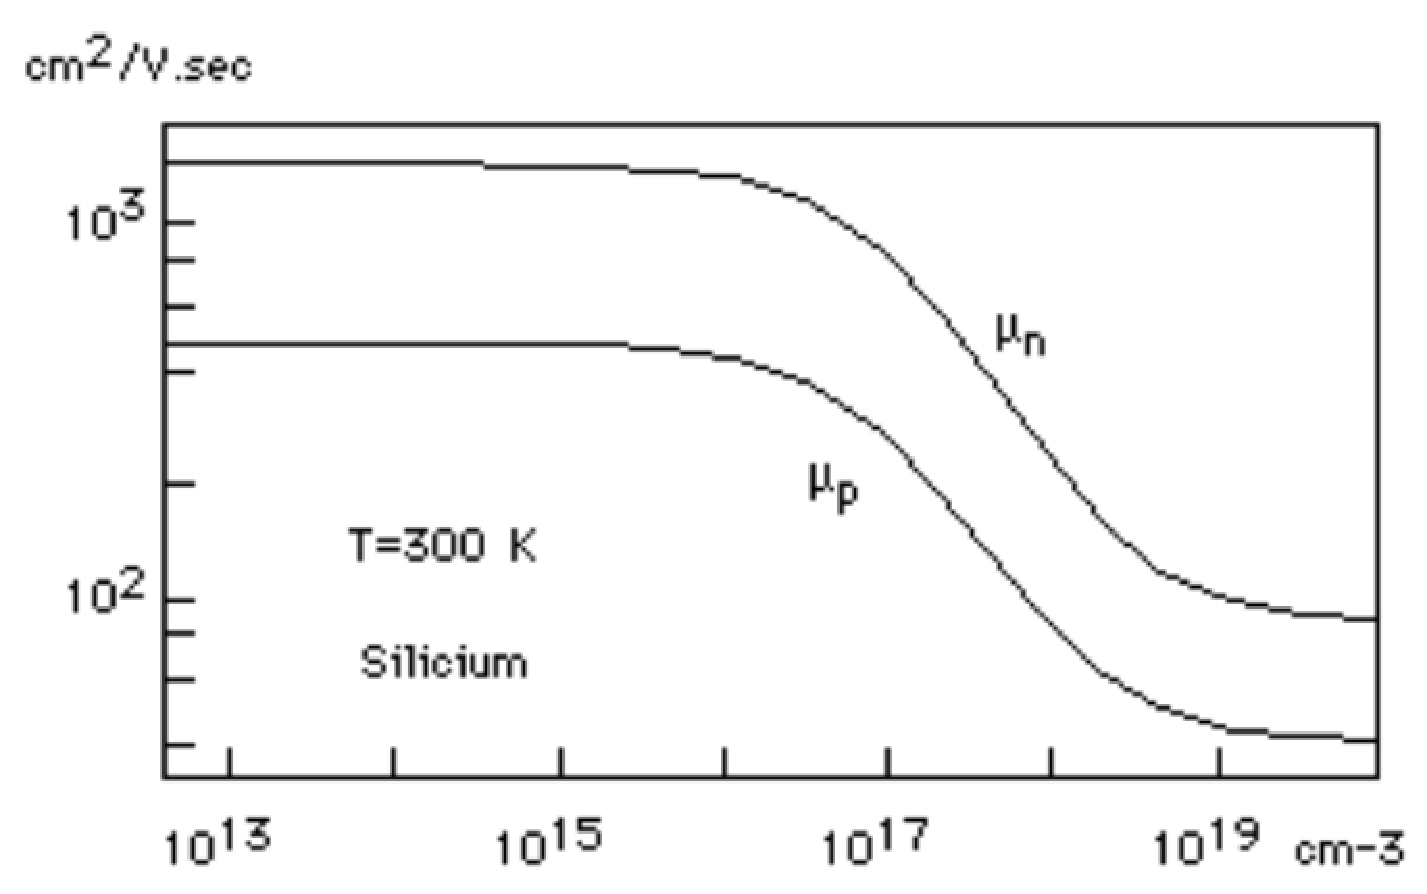
\includegraphics[scale=0.3]{muc.eps} 
%------------------------
\section{Question 8}
Décrire, d'abord qualitativement, puis quantitativement, l'effet Hall. En quoi peut-il être utile pour caractériser un semiconducteur ?
\\
\hbox{\raisebox{0.4em}{\vrule depth 0pt height 0.4pt width 6cm}}
\\
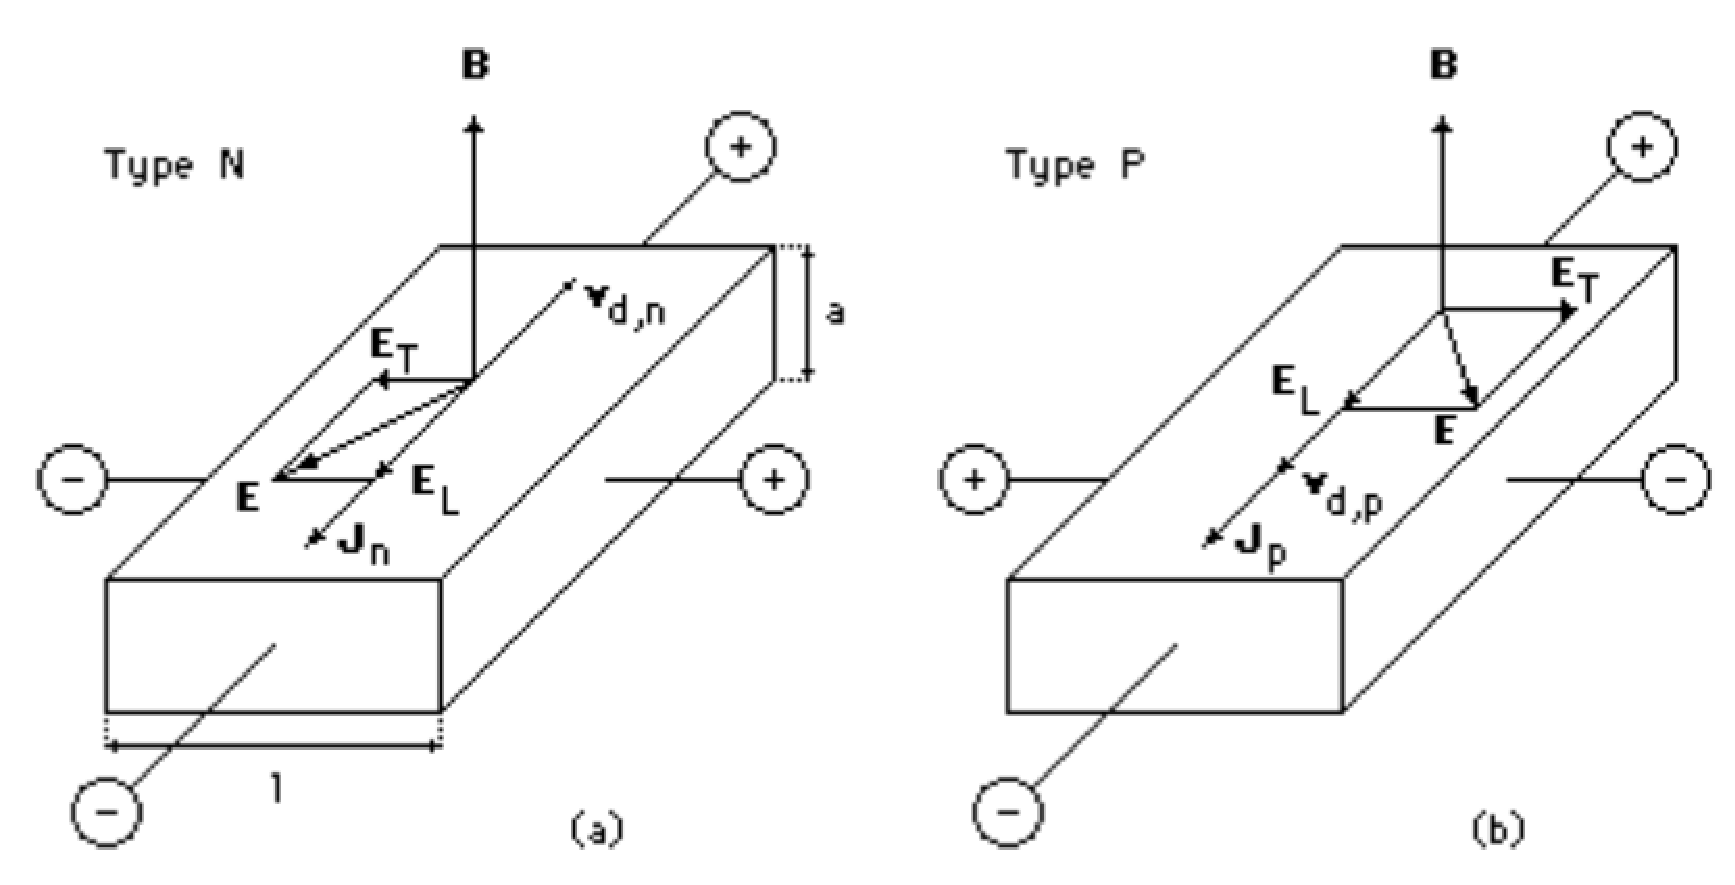
\includegraphics[scale=0.3]{hall.eps} \\
L'effet hall est l'apparition d'une force électromotrice dans un conducteur ou un semi-conducteur lorsque l'on applique un champ magnétique $\mathbf{B}$ perpendiculaire au courant qui le traverse. La force électromotrice est elle même perpendiculaire à ce champ magnétique et à ce courant. Cet effet est dû à la force de Lorenz qui, par l'intermédiaire du champ magnétique, exerce un force sur les charges en mouvement. Ainsi, la densité de charge devient plus grande d'un côté du conducteur et, en réaction, il apparait un champ électrique $\mathbf{E_t} $ qui va s'opposer à ce déplacement de charges.\\
Soit un semi-conducteur de type N (on suppose donc un courant d'électrons), la densité de charge due au courant \textbf{I} est donnée par : 
\begin{equation}
\mathbf{J_n}=-qn\mathbf{V_n}
\end{equation}
Avec n le nombre de porteurs libres et $\mathbf{V_n}$ la vitesse de ces porteurs. La force de Lorenz est donnée dans un champ \textbf{B} par :
\begin{equation}
\textbf{F}=-q(\mathbf{V_n} \times \textbf{B})
\end{equation}
Comme le courant est nul dans la direction perpendiculaire à \textbf{I}, le champ électrique $\mathbf{E_t}$ est égal au champ qui compense la force \textbf{F}, c'est à dire :
\begin{equation}
\mathbf{E_t}=\mathbf{V_n} \times \textbf{B}
\end{equation}
Si l'échantillon a une longueur $l$ et une épaisseur $a$, on définit $V_H$ la tension de Hall, $R_{H,n}$ le coefficient de Hall pour les électrons et $R_{H,p}$ le coefficient de Hall pour les trous : 
\begin{equation}
V_H=lE_t ~~~~~~~et ~~~~~~ R_{H,n} \eqdef \frac{aV_H}{I.B} =\frac{E_t}{J_n.B}=\frac{-1}{qn} ~~~~~~ et ~~~~~~ R_{H,p}=\frac{E_t}{J_pB}=\frac{1}{qp}
\end{equation}
Ainsi, le signe du coefficient de Hall permet de savoir le type (N ou P) de semi-conducteur que l'on a ainsi que sa concentration.

De plus, une mesure de la conductivité permet de connaître la mobilité $\mu$ des porteurs. En effet :
\begin{equation}
\sigma _n =qn\mu _n ~~~~~~~et ~~~~~~ \sigma _p=qp\mu _p
\end{equation}
Et donc :
\begin{equation}
R_{H,n}\sigma _n=-\mu _n ~~~~~~~et ~~~~~~ R_{H,p}\sigma _p=+\mu _p 
\end{equation}

Inversement, si le coefficient de Hall est connu, on peut déterminer l'intensité du champ magnétique appliqué en mesurant la valeur de la tension de Hall.
%----------------------------------------------
\section{Question 9}
Expliquer la différence entre recombinaison Auger et directe radiative. Dans quelles situations les recombinaisons Auger dominent-elles les recombinaisons directes radiatives?
\\
\hbox{\raisebox{0.4em}{\vrule depth 0pt height 0.4pt width 6cm}}
\\
Dans la recombinaison radiative, l'énergie libérée par la transition directe d'un électron d'une bande de conduction vers la bande de valence est dissipée sous forme d'un photon, d'énergie donnée $h\nu $. Le taux net de recombinaison directe $U_d$ est :
\begin{equation}
U_d=c(pn-n_i^2)
\end{equation}
Dans la recombinaison Auger l'énergie perdue lors de la transition est transmise à un autre électron ou à un trou. Le taux net de recombinaison $U_a$ est :
\begin{equation}
U_a=c_1(n^2p-n_i^2n_0)+c_2(p^2n-n_i^2p_0)
\end{equation}
Les 2 types de recombinaison ne sont importants que dans des dispositifs très fortement dopés. La recombinaison Auger prédomine pour les plus hautes valeurs de dopage (dispositifs de puissance). Dans les deux cas, on peut obtenir les temps de vie des porteurs par la formule suivante :
\begin{equation}
\begin{array}{cc}
\tau_n=\frac{n-n_0}{U} & \tau_p=\frac{p-p_0}{U} 
\end{array} 
\end{equation}
Ce qui donne graphiquement le temps de vie des porteurs en fonction du niveau de Fermi :\\
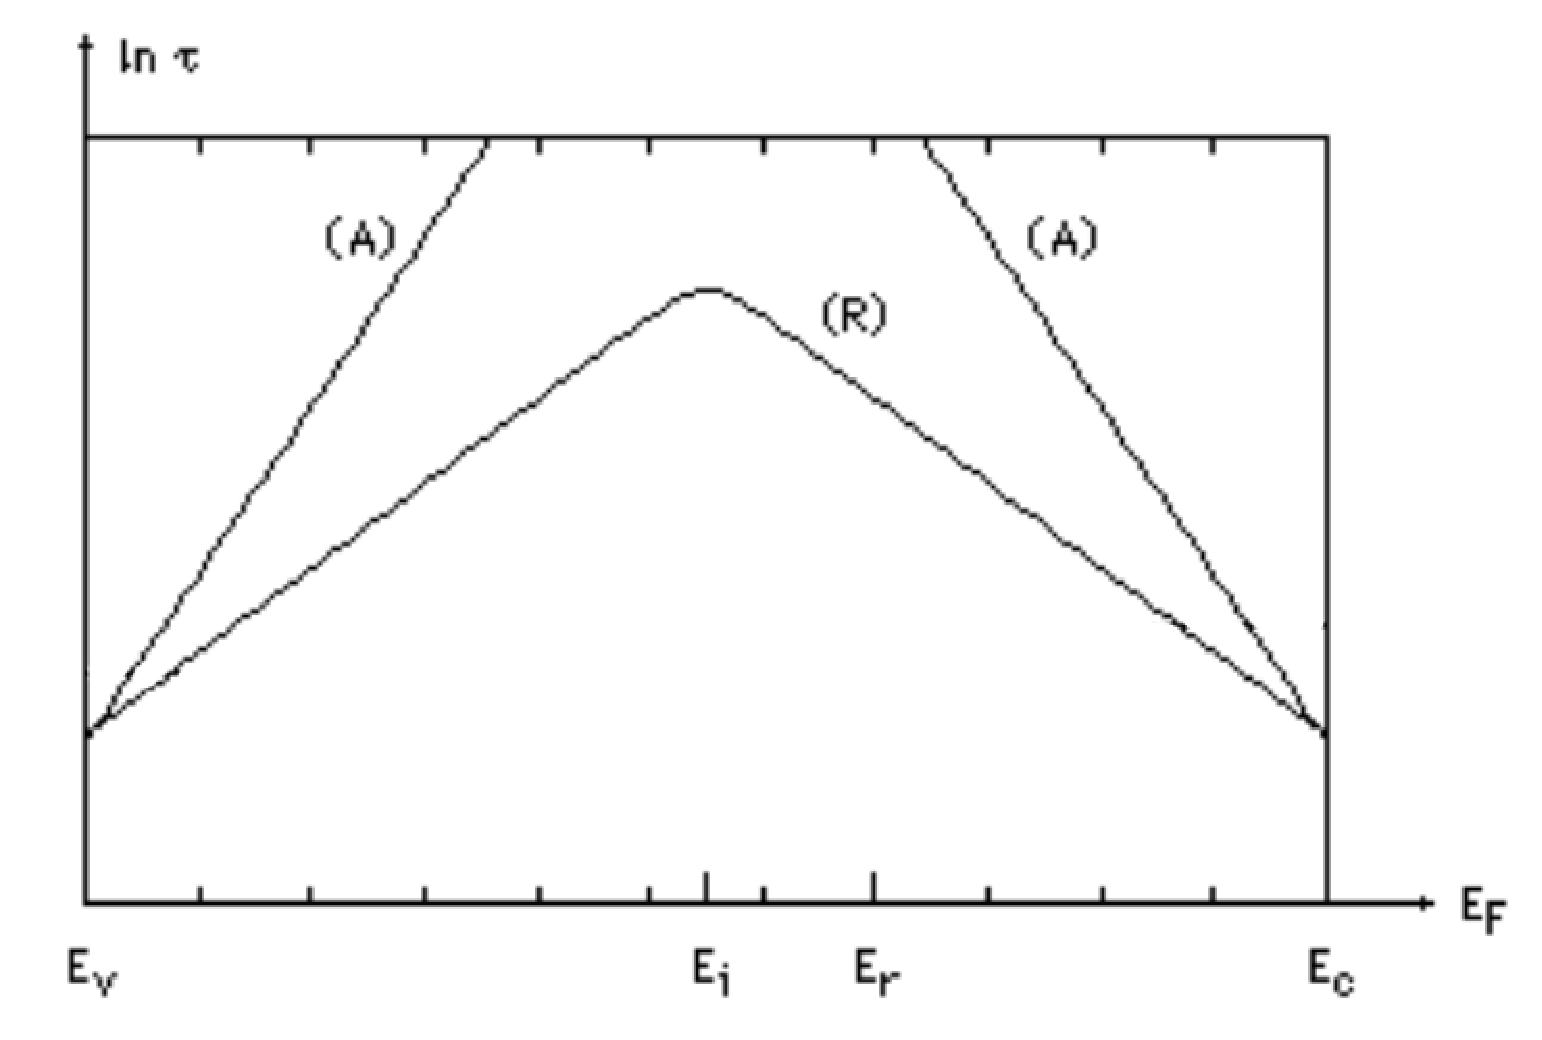
\includegraphics[scale=0.3]{rec.eps} 
%--------------------------------
\section{Question 10}
Décrire brièvement les 3 types de recombinaison dans un semi-conducteur ? Représenter
un graphe du temps de relaxation en fonction du niveau de Fermi pour les 3 types. Dériver mathématiquement les expressions d'une recombinaison, au choix.
\\
\hbox{\raisebox{0.4em}{\vrule depth 0pt height 0.4pt width 6cm}}
\\
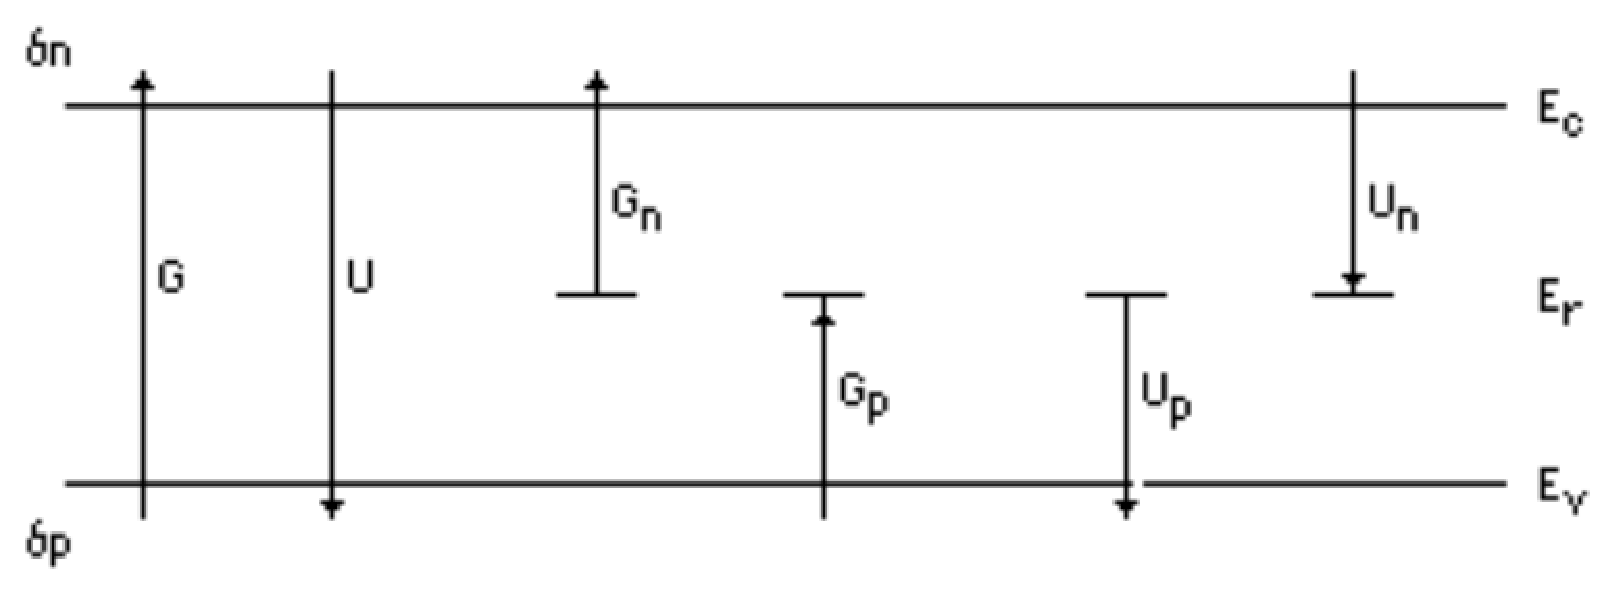
\includegraphics[scale=0.3]{band.eps} \\
Les trois type de recombinaison sont les recombinaisons indirectes (où l'énergie est libérée sous forme de phonon), directes radiative, et Auger. La recombinaison indirecte s'effectue à l'aide de centres de recombinaison qui sont des centres extrinsèques et qui se trouvent proches du milieu de la bande interdite. 
Le taux de recombinaison des trous $U_p$ et des électron $U_n$ est donné par :
\begin{equation}
\begin{array}{cc}
U_n=c_n[n(N_r-n_r)-n_rn_1] & U_p=c_p[pn_r-(N_r-n_r)p_1] 
\end{array} 
\end{equation}
Avec $n_r$/$n_p$ la concentration en électrons/trous qui occupent les centres de recombinaisons d'énergie $E_r$ en concentration $N_r$. Les concentrations $n_1$ et $n_2$ sont données par :
\begin{equation}
\begin{array}{ccc}
n_1=n_i ~exp\left(\frac{E_{r0}-E_{i0}}{kT}\right) & p_1=n_i ~exp\left(-\frac{E_{r0}-E_{i0}}{kT}\right) & n_1p_1=n_i^2
\end{array} 
\end{equation}
La recombinaison est radiative quand l'énergie est libérée lors de la recombinaison l'est sous forme de photon. Le taux net de recombinaison directe $U_d$ est :
\begin{equation}
U_d=c(pn-n_i^2)
\end{equation}
Finalement, elle sera de type Auger si l'énergie libérée par le recombinaison sert à exciter un autre électron ou un trou. 
Le taux net de recombinaison $U_a$ est :
\begin{equation}
U_c=c_1(n^2p-n_i^2n_0)+c_2(p^2n-n_i^2p_0)
\end{equation}
Dans les trois cas, le temps de vite des électrons et des trous est donné par :
\begin{equation}
\begin{array}{cc}
\tau_n=\frac{n-n_0}{U} & \tau_p=\frac{p-p_0}{U} 
\end{array} 
\end{equation}
Graphe du temps de relaxation en fonction du niveau de Fermi pour les 3 types\\
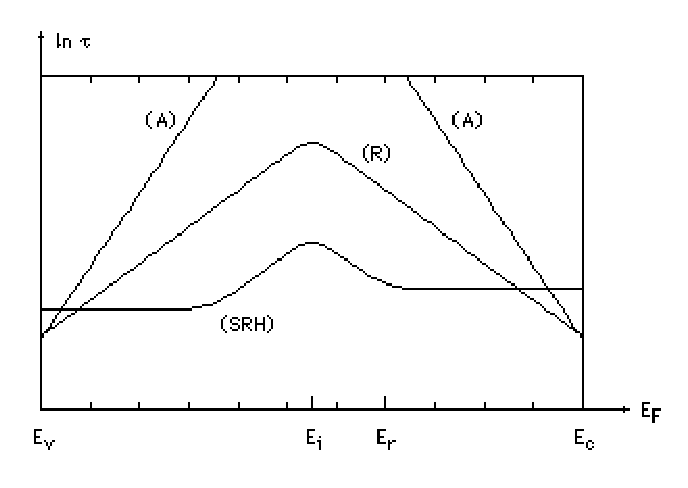
\includegraphics[scale=1]{recomb.eps} \\
Pour des dopages faibles, on a surtout de la recombinaison indirecte, les recombinaisons radiatives et Auger ne deviennent importantes que pour des dispositifs fortement dopés.\\
\subsection{recombinaison indirecte}
Calcul des taux de recombinaison $U_n$ et $U_p$ pour une recombinaison indirecte, par l'intermédiaire de centres de recombinaison d'énergie $E_r$. La concentration de ces centres est $N_r$ (supposés de type accepteur), et $n_r$ la concentration d'électrons qui occupent ces centres. (Le résultat qui sera obtenu est également valable pour les sites de type donneur).\\
Le taux de recombinaison $U_n$ est la différence de deux contributions :
\begin{enumerate}
\item Le taux $U_{n,a}$ de capture d'électrons libres de la bande de conduction dans un centre neutre de recombinaison
\item Le taux $U_{n,b}$ de génération thermique des centres négatifs vers la bande de conduction.
\end{enumerate}
Le taux de capture d'électron $U_{n,a}$ est proportionnel au nombre $n$ d'électrons dans la bande de conduction, ainsi qu'au nombre $(N_r-n_r)$ de centres vides : 
\begin{equation}
U_{n,a}=c_n n (N_r-n_r)
\end{equation}
avec $c_n$ un coefficient qui prend en compte la probabilité de capturer un électron libre par un centre de recombinaison. \\
Le taux de génération thermique $U_{n,b}$ est proportionnel au nombre de centres négatifs $n_r$ et au nombres de places libres dans la bande de conduction $p_c$ :
\begin{equation}
U_{n,b}=e_nn_rp_c
\end{equation}
où $e_n$ est un coefficient de probabilité de passage d'une bande à l'autre en fonction de la température. On réécrit cependant cette expression sous la forme :
\begin{equation}
U_{n,b}=c_nn_rn_1
\end{equation}
On obtient ainsi un taux net $U_n$ donné par :
\begin{equation}
U_n=c_n[n(N_r-n_r)-n_rn_1]
\end{equation}
On obtient par un raisonnement similaire $U_p$ :
\begin{equation}
U_p=c_p[pn_r-(N_r-n_r)p_1] 
\end{equation}
On peut alors calculer les termes $n_1$ et $p_1$ en considérant l'équilibre thermodynamique pour lequel $U_n=U_p=0$
\begin{equation}
\begin{array}{c}
U_n=c_n[n_0(N_r-n_{r0})-n_{r0}n_1]=0 \Rightarrow n_1=\frac{n_0(N_r-n_{r0})}{n_{r0}}
\\ 
U_p=c_p[p_0n_{r0}-(N_r-n_{r0})p_1] =0 \Rightarrow p_1=\frac{p_0n_{r0}}{(N_r-n_{r0})}
\end{array} 
\end{equation}
Dans lesquels on peut substituer les expressions d'équilibre :
\begin{equation}
\begin{array}{c}
n_0=n_i exp\left( \frac{E_f-E_{io}}{kT}\right)~exp\left( \frac{q\phi_0}{kT}\right)\\
p_0=n_i exp\left( \frac{E_{io}-E_f}{kT}\right)~exp\left( \frac{-q\phi_0}{kT}\right)\\
n_{r0}=\frac{N_r}{1+exp\left( \frac{E_{ro}-E_f}{kT}\right)~exp\left( \frac{-q\phi_0}{kT}\right)} \\
\end{array} 
\end{equation}
Et on obtient alors les expressions suivantes :
\begin{equation}
\begin{array}{ccc}
n_1=n_i ~exp\left(\frac{E_{r0}-E_{i0}}{kT}\right) & p_1=n_i ~exp\left(-\frac{E_{r0}-E_{i0}}{kT}\right) & n_1p_1=n_i^2
\end{array} 
\end{equation}
\subsection{recombinaison directe radiative}
Le taux net de recombinaison directe U doit être proportionnel à la densité de porteurs n et p, et dépend de la génération thermique $U_b$ (qui va diminuer le taux net de recombinaison). On obtient donc une équation de la forme suivante : 
\begin{equation}
U=cnp-U_b
\end{equation}
On sait qu'à l'équilibre thermodynamique, $U$ doit être nul. On peut ainsi calculer $U_b=cnp$. Or, à l'équilibre, on a $n=p=n_i$; on a alors:
\begin{equation}
U_b=cn_i^2 \Rightarrow U=c(np-n_i^2)
\end{equation}
On calcule alors facilement les durées de vie des porteurs correspondants :
\begin{equation}
U_n=\frac{n-n_0}{\tau _n} \Rightarrow \tau _n=\frac{n-n_0}{c(np-n_i^2)}
\end{equation} 
\begin{equation}
U_p=\frac{p-p_0}{\tau _p} \Rightarrow \tau _p=\frac{p-p_0}{c(np-n_i^2)}
\end{equation} 
\subsection{recombinaison Auger}
Le taux net de recombinaison Auger fait intervenir 3 particules, soit 2 électrons et un trou, soit 2 trous et un électron et la taux net de recombinaison serra proportionnel à leur concentration. Le taux de recombinaison fera également intervenir la génération thermique $U_b$ qui va diminuer le taux net de recombinaison. On obtient donc une équation de la forme suivante : 
\begin{equation}
U=c_1n^2p+c_2p^2n-U_b
\end{equation}
On peut calculer le terme de recombinaison thermique $U_b$, sachant que $U=0$ à l'équilibre thermodynamique avec $n_0=p_0=n_i$:
\begin{equation}
c_1n_0^2p_0+c_2p_0^2n_0-U_b=0 \Rightarrow U_b=(c_1n_0+c_2p_0)n_i^2
\end{equation}
On obtient donc :
\begin{equation}
U=c_1(n^2p-n_i^2n_0)+c_2(p^2n-n_i^2p_0)
\end{equation}
\subsection{supplément : Faible injection}
Dans les trois cas, on peut faire l'hypothèse de faible injection. C'est à dire qu'il existe un faible excès de porteurs par rapport à l'équilibre :
\begin{equation}
\begin{array}{c}
\delta n=n-n_0 \ll n_0 ~ou~ p_0 \\
\delta p=p-p_0 \ll p_0 ~ou~ n_0 \\
\end{array} 
\end{equation}
On fait aussi généralement l'approximation que $\delta n=\delta p$.
%------------------------------------------------
\section{Question 11}
Justifiez , d'abord qualitativement, et ensuite par un développement mathématique,
l'hypothèse de neutralité électrique locale dans un semi-conducteur dopé N de manière
homogène. Pour cela, montrez comment évolue dans le temps une faible perturbation locale de la densité de charge.
\\
\hbox{\raisebox{0.4em}{\vrule depth 0pt height 0.4pt width 6cm}}
\\
Si on applique une faible perturbation de la densité de charges, il va apparaitre un champ électrique, qui va provoquer la dérive des porteurs majoritaires, ce qui va neutraliser la charge excédentaire après un bref laps de temps (transitoire). Après quoi le semi-conducteur est à nouveau homogène. 
Mathématiquement, considérons que la perturbation ait lieu à $t_0$ et consiste en un excès de charge positive, dans un semi-conducteur de type N (est donc $n_0>>p_0$). Soit $p_0$ et $n_0$ les concentrations initiales et $p=p(x,t)$ la concentration de trous après la perturbation. Comme on a une faible perturbation, $p$ varie peu de $p_0$, et donc, on a $p<<n_0$.On remarque aussi que $n$ sera quasi égal à $n_0$ (en effet si l'équilibre est respecté on a $n=N_D+p=p+n_0-p_0 \approx n_0$) La charge d'espace $\rho$ est donnée par la somme des charges des porteurs :
\begin{equation}
\rho =q(p-n+N_D)
\end{equation}
Si on travaille en une seule dimension, le champ électrique est donné par :
\begin{equation}
\frac{\partial E}{\partial x}=\frac{\rho}{\epsilon _s} 
\end{equation}
On cherche à montrer que le temps pour revenir à le neutralité est très court; on peut donc négliger les phénomènes de recombinaison et de diffusion des porteurs qui auront des temps caractéristiques plus grands. Les courants de dérive générés pas ce champ électrique sont donnés par :
\begin{equation}
J_n=qn\mu _n E~~~~~~ et ~~~~ J_p=qp\mu _p E 
\end{equation}
Avec les hypothèses ci-dessus, on a que $J_n \gg J_p$ et donc que $J=J_n+J_p \approx J_n$\\
Avec les conditions aux limites on a, en utilisant les hypothèses simplificatrices:
\begin{equation}
\frac{\partial n}{\partial t}=\frac{1}{q}\frac{\partial J_n}{\partial x}
\end{equation} 
\begin{equation}
\frac{\partial p}{\partial t}=\frac{-1}{q}\frac{\partial J_p}{\partial x}
\end{equation}
La différence de ces deux équations donne alors :
\begin{equation}
-\frac{\partial (p-n)}{\partial t}=\frac{1}{q}\frac{\partial (J_p+J_n)}{\partial x} \approx \frac{1}{q}\frac{\partial (J_n)}{\partial x} = n_0\mu _n \frac{\partial (E)}{\partial x}
\end{equation}
On utilise alors $\frac{\rho}{q}-N_d=(p-n)$ et $\sigma=q(n\mu _n+p\mu _p) \approx q n_0 \mu _n$ on a :
\begin{equation}
\frac{\partial (\rho)}{\partial t}=-\frac{\sigma}{\epsilon _s} \rho 
\end{equation}
La solution à cette équation est alors :
\begin{equation}
\rho =\rho _0 e^{(- \sigma t/\epsilon _s)}
\end{equation}
La solution montre que le retour à l'équilibre après une faible perturbation s'effectue selon une fonction exponentielle décroissante du temps. La constante de temps de l'exponentielle est $\epsilon _s / \sigma$, ce qui est de l'ordre de $10^{-12}s$. Le retour à l'équilibre est donc très rapide. Ceci justifie, à postériori, les approximations faites. En effet, à ces échelles de temps, la recombinaison et la diffusion sont pratiquement inactives.

\end{document}
